%% Version 6.1, 1 September 2021
%
%%%%%%%%%%%%%%%%%%%%%%%%%%%%%%%%%%%%%%%%%%%%%%%%%%%%%%%%%%%%%%%%%%%%%%
% TemplateV6.1.tex --  LaTeX-based blank template for submissions to the 
% American Meteorological Society
%
%%%%%%%%%%%%%%%%%%%%%%%%%%%%%%%%%%%%%%%%%%%%%%%%%%%%%%%%%%%%%%%%%%%%%
% PREAMBLE
%%%%%%%%%%%%%%%%%%%%%%%%%%%%%%%%%%%%%%%%%%%%%%%%%%%%%%%%%%%%%%%%%%%%%

%% Start with one of the following:
% 1.5-SPACED VERSION FOR SUBMISSION TO THE AMS
\documentclass{ametsocV6.1}
\usepackage{subcaption}
\usepackage{float}
\usepackage{amsmath}
% TWO-COLUMN JOURNAL PAGE LAYOUT---FOR AUTHOR USE ONLY
%\documentclass[twocol]{ametsocV6.1}

%%%%%%%%%%%%%%%%%%%%%%%%%%%%%%%%

%%% To be entered by author:

%% May use \\ to break lines in title:

\title{Towards operational deep-learning downscaling: Improving GAN downscaling of temperature, humidity and precipitation}

%% Enter authors' names and affiliations as you see in the examples below.
%
%% Use \correspondingauthor{} and \thanks{} (\thanks command to be used for affiliations footnotes, 
%% such as current affiliation, additional affiliation, deceased, co-first authors, etc.)
%% immediately following the appropriate author.
%
%% Note that the \correspondingauthor{} command is NECESSARY.
%% The \thanks{} commands are OPTIONAL.
%
%% Enter affiliations within the \affiliation{} field. Use \aff{#} to indicate the affiliation letter at both the
%% affiliation and at each author's name. Use \\ to insert line breaks to place each affiliation on its own line.

%\authors{Author One,\aff{a}\correspondingauthor{Author One, email@email.com} 
%Author Two,\aff{a} 
%Author Three,\aff{b} 
%Author Four,\aff{a} 
%Author Five\thanks{Author Five's current affiliation: NCAR, Boulder, Colorado},\aff{c} 
%Author Six,\aff{c} 
%Author Seven,\aff{d}
% and Author Eight\aff{a,d}
%}
%
%\affiliation{\aff{a}{First Affiliation}\\
%\aff{b}{Second Affiliation}\\
%\aff{c}{Third Affiliation}\\
%\aff{d}{Fourth Affiliation}
%}

\authors{Kiri Daust\aff{a,b}\correspondingauthor{Kiri Daust, kiridaust@uvic.ca}, Adam Monahan\aff{a},Colin Mahony\aff{b}}

\affiliation{\aff{a}{University of Victoria}\\
\aff{b}{Future Forest Ecosystem Centre, BC Ministry of Forests}
}

%%%%%%%%%%%%%%%%%%%%%%%%%%%%%%%%%%%%%%%%%%%%%%%%%%%%%%%%%%%%%%%%%%%%%
% ABSTRACT
%
% Enter your abstract here
% Abstracts should not exceed 250 words in length!
%
 
\abstract{}

\begin{document}

%% Necessary!
\maketitle


%%%%%%%%%%%%%%%%%%%%%%%%%%%%%%%%%%%%%%%%%%%%%%%%%%%%%%%%%%%%%%%%%%%%%
% MAIN BODY OF PAPER
%%%%%%%%%%%%%%%%%%%%%%%%%%%%%%%%%%%%%%%%%%%%%%%%%%%%%%%%%%%%%%%%%%%%%
%

%% In all cases, if there is only one entry of this type within
%% the higher level heading, use the star form: 
%%
% \section{Section title}
% \subsection*{subsection}
% text...
% \section{Section title}

%vs

% \section{Section title}
% \subsection{subsection one}
% text...
% \subsection{subsection two}
% \section{Section title}

%%%
% \section{First primary heading}

% \subsection{First secondary heading}

% \subsubsection{First tertiary heading}

% \paragraph{First quaternary heading}

\section{Introduction}
Accurate, local-scale climate information is essential support for societal efforts to adapt to rapid climate changes. Earth System Models (ESMs) provide state-of-the-art projections on a global scale, but at insufficient spatial resolution for local planning. Thus, downscaling - creating high-resolution climate information from low-resolution, large-scale model output - is an important practical tool for planning and decision making. Spatially and temporally high resolution fields of climate data over large scales are important for many applications, including simulation of extreme events at local scales \citep[e.g. fires, floods, storms;][]{fischer2021increasing}, local infrastructure planning, and making climate informed ecological decisions such as tree species selection \citep{mackenzie2021ecological}. Unfortunately, accurate downscaling is often limited by computational constraints. Ideally, we would like downscaling techniques to be computationally efficient, accurate over regions with different climates, and capable of capturing extremes. The latter requirement also suggests that we should be able to generate ensembles of downscaled fields, to sample the full range of meteorological states.

Strategies for downscaling coarse-resolution climate model simulations to regional scales can be broadly classified into dynamic downscaling and statistical downscaling. Dynamic downscaling employs a limited-area numerical climate model to resolve fine-scale features,  driven by large-scale weather patterns from the low resolution ESM \citep{skamarock2001prototypes}. Statistical downscaling develops statistical relationships between low-resolution (LR) and high-resolution (HR) climate variables, using a variety of strategies including regression, interpolation, cluster analysis, lapse rate adjustment, and gaussian process/kriging (ref xxx colin). Both downscaling approaches have strengths and weaknesses. 

Dynamical downscaling is generally more accurate at capturing fine-scale spatial patterns (e.g., rainshadow effects, elevation dependant warming) than statistical downscaling, as it uses physical models of the atmosphere. It can be implemented at multiple spatial scales, and different classes of downscaling often lend themselves to different model specifications. Regional climate models (RCMs) have existed for decades, and are usually used to downscale ESM or reanalysis products to a 20-40 km resolution. For many of the applications discussed above, it is beneficial to have finer spatial resolution. Convection permitting models usually operate on a 1 - 4 km resolution, and can much more accurately represent weather patterns do to simulated some fine scale convection processes. However, due to their computation expense, they are of limited use for exploring climate change uncertainty, and are often not practical for operational products.

Statistical downscaling is generally much more computationally efficient than dynamical downscaling, but can have limited capacity to downscale variables with complex dependence structures. Also, traditional statistical downscaling usually requires observations to calibrate models properly. Over the past few years, deep-learning has been introduced as a new statistical downscaling strategy which can potentially capitalise on the benefits of both traditional statistical and dynamical downscaling. Specifically, deep neural networks can be trained on HR output from dynamic downscaling, and the network learns to ``emulate" the dynamic downscaling, given a suite of LR climate information. This paper focuses on stochastic ensemble downscaling, where the deep-learning model attempts to learn the conditional distribution of the HR fields, and then sample realisations from those. In this framework, the LR climate input are then the conditioning fields, since they condition the distribution that the model attempts to learn. So far, deep-learning methods have demonstrated potential for creating downscalings of similar quality to dynamic methods, but with the efficiency of standard statistical methods (ref xxx). The deep-learning downscaling we present in this paper attempts to emulate the results of convection permitting models, downscaling to high spatial resolution at hourly timesteps. 

Most of the recent research in generative deep-learning based downscaling has employed conditional Generative Adversarial Networks (GANs). GANs, first introduced by \citet{goodfellow2014generative} and adapted into a conditional version by \citet{mirza2014conditional}, contain two deep convolutional networks, the Generator and the Critic. During training, these networks compete; the Generator tries to fool the Critic by producing output similar to the training data, and the Critic tries to distinguish between real and generated samples. Theoretically, the GAN will learn to sample from the conditional distribution of the HR variables, conditioned on the LR fields. \citet{annau2023algorithmic} developed a GAN framework which produced accurate downscaling of wind components. Recent work by \citet{daust2024capturing} adapted this framework to be fully stochastic, allowing the GAN to sample multiple realisations from the learned conditional distribution. Their study showed that when applied to downscaling wind components, the stochastic GAN was well calibrated and was better at predicting extremes. This current work uses the basic network architecture developed by \citet{annau2023algorithmic} and then adapted to be fully stochastic in \citet{daust2024capturing}. 

While substantial research has investigated GAN downscaling, there multiple questions that should still be addressed prior to use in an operational setting. First, most studies to date have focused on downscaling single variables. Many studies \citep[e.g.,][]{harris2022generative,leinonen2020stochastic,price2022increasing} have focused on precipitation, and while \citet{annau2023algorithmic} and \citet{daust2024capturing} employed multivariate GANs, they focused solely on downscaling wind components. However, operational downscaling is often required to provide a suite of variables. Temperature, humidity, precipitation, and wind are essential variables for a broad range of applications including fire weather, hydrology, ecology, and urban planning. While the stochastic GAN developed in \citet{daust2024capturing} produced accurate downscaling of wind components, its ability to extend to other variables has not previously been assessed. Multiple studies \citep{harris2022generative,leinonen2020stochastic} have shown that GANs can struggle to capture extreme precipitation events, a task which is crucial for adaptation planning (ref xxx importance of extremes). \citet{daust2024capturing} found that their stochastic GAN was better at capturing extremes in wind components than an equivalent deterministic model. Since many traditional statistical downscaling methods succeed for means, but struggle to capture extremes, it will be important to ascertain the extent to which GAN downscaling can capture important extremes. 

Downscaling of multiple climate variables invites the possibility of using fully multivariate GANs, where multiple variables are predicted from one model. Such an approach could improve dependence structures between variables, especially at small scales. While some dependence between variables will be inherited from the LR conditioning fields, multivariate models may be able to create correct dependence of fine-scale generated features, leading to improved consistency. However, most studies so far have only used univariate GANs \citep{harris2022generative,leinonen2020stochastic,price2022increasing}, and while \citet{annau2023algorithmic} and \citet{daust2024capturing} showed success with multivariate downscaling of wind components, it is uncertain what the costs and benefits of multivariate prediction might be when extended to more variables. Wind components are very closely physically linked with similar distributions and dependence structures, are are not a very challenging multivariate downscaling problem. From an operational perspective, multivariate GAN downscaling is desirable, as it decreases the number of models requiring training. 

Commonly, GANs used in downscaling research input all the conditioning information (i.e., covariates) at LR. While this is necessary for variables coming from LR models, there is often pertinent surface information (such as topography) available at high resolution. Intuitively, providing surface information at a higher resolution should improve the performance of the model. However this hypothesis has not been systematically tested, and it requires adjusting the architecture of the Generator network from that using only LR covariates. \citet{harris2022generative} included HR topography information by first convolving it down to LR and then concatenating with the climate variables - essentially trying to fit more information into the LR architecture. \citet{daust2024capturing} used a different approach with two parallel Generator streams for covariates of different resolution. It is important to assess how these architectural changes impact the results.

Most studies investigating GAN downscaling use small domains for computational reasons, and the ability of GAN frameworks to generalise over large spatial reasons has yet to be assessed. Applying GAN downscaling over large contiguous areas poses many challenges. Computational constraints aside, it is unclear whether a single GAN framework can optimally downscale the idiosyncratic weather of disparate regions in a large study area, as most research to-date has developed and tested GAN frameworks in a single region. Showing that a GAN framework can generalise over space is a first step to developing models capable of downscaling large regions.

This current study aims to address these some of these questions and investigate the applicability of stochastic GANs to future operational downscaling. Specifically, we apply the stochastic GAN framework to temperature, humidity, precipitation, as well as both wind components. Initial analyses are conducted in the region of complex topography (include Vancouver Island, the Coast Mountains, and the Interior Plateau on the Pacific Northwest of North America) considered by \citet{daust2024capturing}. We then investigate the advantages and disadvantages of univariate versus multivariate prediction. The paper then assesses the utility of providing HR topography to the GAN. Finally, we test the GAN framework on all five variables in a second region in Northeastern British Columbia and Alberta (a region with relatively flat topography) and assess the spatial generalisability of the GAN framework.

\section{Methods}
All GANs in this paper use the same basic structure. We train the models on paired sets of LR conditioning fields (covariates), time-invariant HR surface features, and HR truth fields. The GAN then learns a mapping to the HR fields from the input covariates. For consistency, we keep the same resolution and size of fields across all models: HR fields are 128x128 pixels (corresponding to approximately 270x450 km or $4^\circ$x$4^\circ$), and LR fields are 16x16 pixels, corresponding to a downscaling factor of eight. 

\subsection{Data}
A natural use of GANs in a downscaling setting involves training on paired HR regional weather model output and LR ESM or reanalysis data. We follow this approach, using ERA5 reanalysis variables as the LR predictors, and a Western Canada Weather Research and Forecasting (WRF) model output \citep{li2019high} as the paired HR training data. The WRF model is a state-of-the-art numerical weather model, designed for convection-permitting scale (3-4 km) forecasts. This specific WRF run was driven by ERA-interim, covers all of British Columbia, and has a 4 km grid-size resolution. We used ERA5 as the paired LR data since it provided all the covariates we planned to use, whereas ERA-interim only provided a subset of them. Although there will be some differences between ERA5 and ERA-Iterim, they represent the same realisation of the climate system so it is reasonable to use ERA5 as the paired LR dataset. However, it is important to note that in this  downscaling scenario, where HR and LR data each come from separate models, there will be large-scale biases between the WRF output and the ERA5 conditioning fields. The WRF model generates internal variability, which will also cause differences between models on common scales. Thus, a successful GAN must learn to bias correct, downscale, and accommodate internal variability.

Unless otherwise noted, the GANs we consider use a suite of seven LR covariates: temperature (2m), specific humidity (2m), precipitation, wind components (10m), convective available potential energy (CAPE) and surface pressure. We also include HR topography as an invariant field. For the majority of our analyses, we consider a rectangular region in Southwestern BC, Canada ($49^\circ$ to $53^\circ$ N, $122^\circ$ to $126^\circ$ W; henceforth called the Southwest region), as its high degree of topographic complexity represents a realistically challenging downscaling scenario (figure \ref{studyarea}). \citet{daust2024capturing} tested stochastic GANs for downscaling wind components in this region; we extend the analysis to downscale temperature, specific humidity, and precipitation. As is common in deep learning we standardise all variables to mean zero and unit standard deviation prior to training. 

To investigate the applicability of this GAN framework to different regions, we also investigate a second region in the northeast of BC and the northwest of Alberta (the Northeast region), which in contrast to the Southwest region has flat topography and is influenced by different weather processes. We also investigate using a land use index, which includes waterbodies and forest types, as a second HR invariant field.

\begin{figure}[H]
  \noindent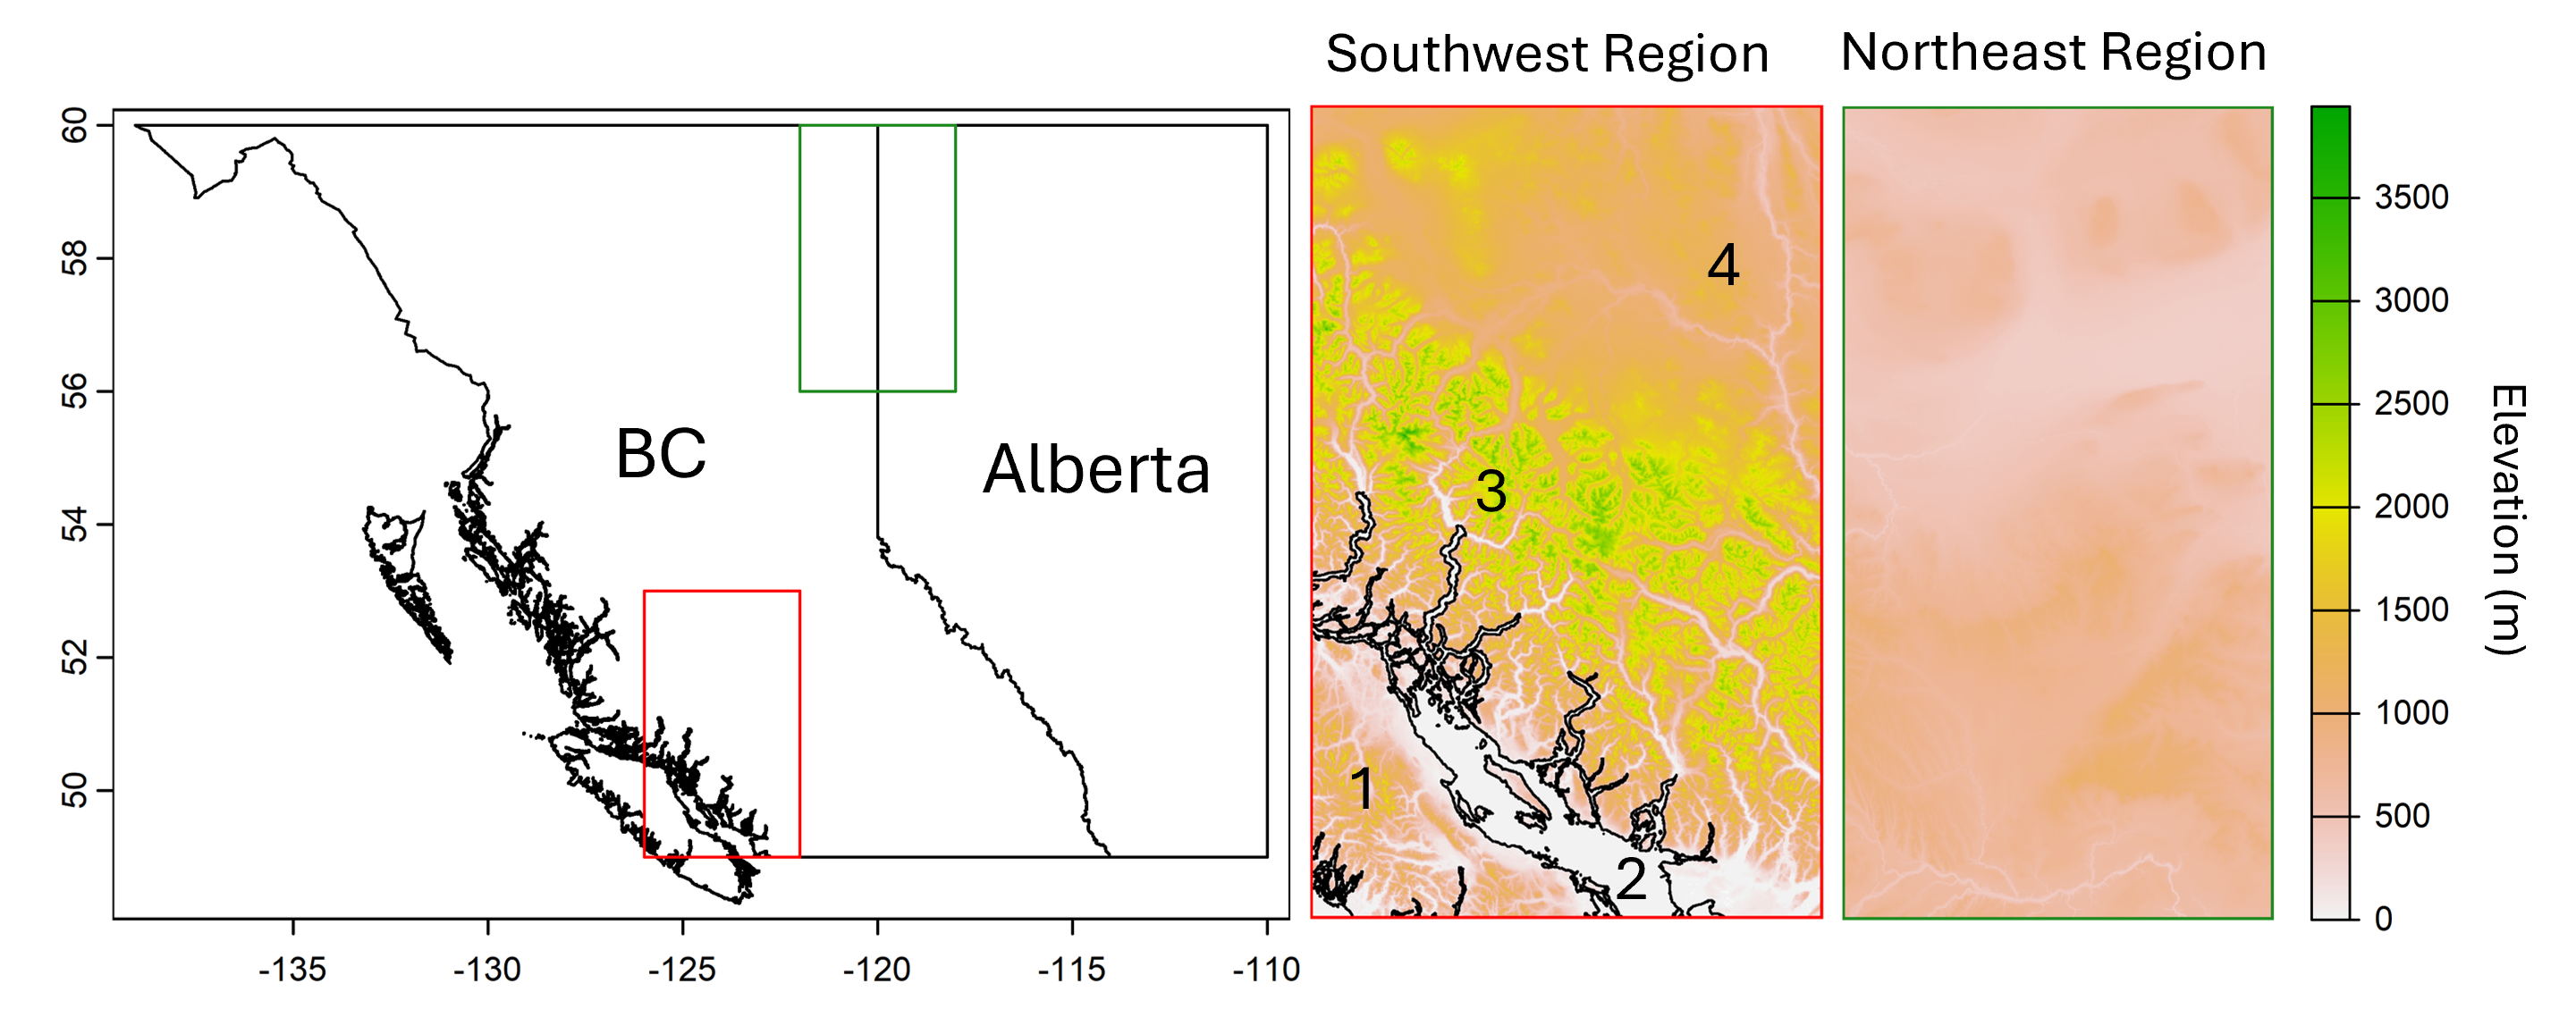
\includegraphics[width=\textwidth,angle=0]{final/StudyAreas.png}\\
  \caption{Maps of study areas, showing (from left to right) study area locations relative to British Columbia and Alberta, and topographic relief of both regions. 1 = Vancouver Island, 2 = Georgia Straight, 3 = Coast Mountains, and 4 = Interior Plateau.}\label{studyarea}
\end{figure}

\subsection{Model}
In the initial GAN formulation, the Critic network estimates the probability of a sample being from the training set; the Generator attempts to make it more challenging to distinguish training samples, while the Critic tries to improve its ability at discriminating. This approach often led to instability during training, as it requires that both networks learn at approximately the same rate and can lead to vanishing gradients (ref xxx). \citet{arjovsky2017wasserstein} addressed this challenge with the introduction of the Wasserstein GAN, where the Critic estimates the Wasserstein distance between the generated and training samples. Intuitively, the Wasserstein distance represents the amount of mass required to transform one distribution to another, and is a distance metric between the distributions. In our case, the Wasserstein distance estimates the distance between the high-dimensional distributions of the training data and the generated output. During training, the Generater attempts to minimize the Wasserstein distance between the generated fields and the training data, thus increasing the distributional similarity between them. Following recent literature in downscaling and computer vision (refs xxx), we adopt this approach. 

One appealing aspect of GANs compared to more standard Convolutional Neural Networks, especially for climate downscaling, is that they do not solely rely on a pixel-wise error metric as the loss function. Downscaling is an underdetermined problem, meaning that there is a distribution on HR fields consistent with a single set of LR conditioning fields. Thus, while we require convergence in large-scale structure between the downscaled results and the LR conditioning fields, we should accept slight differences in fine-scale structure between the generated output and the training data. Using a pixelwise metric such as mean absolute error can overly constrain models by forcing them to match the training data too closely, a phenomenon known as the double-penalty problem. In such cases, the model will often converge on the conditional median, producing blurry output. In contrast, the adversarial loss calculated by the GAN's Critic network (in our case, the Wasserstein distance) is not a pixel-wise metric, and aims for convergence in distribution, which is a desireable property. However, \citet{wang2018esrgan} showed that only using the adversarial loss in the Generator training procedure often leads to unstable training and poor convergence of large-scale structures. They suggested adding a pixel-wise loss back in as the content-loss, to reward convergence in realisation at large-scales. We follow this approach, and our Generator loss function is composed of both the adversarial loss, and a pixel-wise content loss. A more detailed discussed of this issue is presented in \citet{annau2023algorithmic}.

This study uses the stochastic GAN architecture developed by \citet{daust2024capturing}, which was based on the deterministic GAN described in \citet{annau2023algorithmic}. The architecture makes extensive use of convolutional layers, which are designed to extract representative features from images \citep{li2021survey}. In the Generator network, we use Residual in Residual Dense Blocks (RRDB), which contain stacked convolutional layers followed by leaky rectified linear units to add non-linearity. For upsampling, we use three pixel-shuffle blocks \citep{shi2016real}. Following \citet{daust2024capturing}, we inject Gaussian noise fields into the convolutional filters inside each RRDB. We also include a HR input stream to allow inclusion of HR covariates, such as topography. This stream uses the same structure of RRDB as that of the LR inputs, but skips the upsampling step. Once the upsampling has occurred on the LR stream, all inputs have the same dimension, and are concatenated. We also include all covariates as inputs to the Critic network, using a LR input stream for the LR covariates. Intuitively, including the conditioning information should allow the Critic to better estimate the conditional distributions. 

Unless otherwise specified, all models presented in this study use the best model from \citet{daust2024capturing}, with stochastic sampling and CRPS as a content loss. Stochastic sampling, adapted from \citet{harris2022generative} creates multiple realisations of each training sample, and computes the content loss across these realisations. CRPS is a probabilistic measure, which aims for convergence in pixelwise distributions. As our aim is to sample from the HR conditional distributions, it is natural to use a probabilistic metric. Since stochastic sampling and the CRPS content loss are only applicable in a stochastic setting, when using a deterministic Generator, we employed standard training with MAE as a content loss, as in \citet{annau2023algorithmic}. 

\subsection{Training}
We trained individual models for each of temperature, specific humidity, and precipitation using the framework described above. We used two years of hourly data as a training set (2003 and 2006), and one year as an out-of-sample test set (2005). Initial tests showed that model results did not improve substantially using more than two years of training data, so we chose this size for computational efficiency. Models were trained until metrics on the test dataset stabilised ($\leq$ 250 epochs). We then saved the Generator from the final epoch for analysis. Multivariate models for predicting all variables were trained in a similar way, with the HR training data created by stacking the individual variables as separate channels. We trained all models on an NVIDIA RTX 4090 GPU; models took on average 48 hours to train.

\citet{daust2024capturing} found that the stochastic GAN was better able to capture wind component extremes (i.e., the tails of the distribution) than the determinstic GAN. A common challenge with precipitation downscaling is underestimation of high-precipitation events \citep{kumar2023modern}. We thus created a deterministic GAN similar to that considered in \citet{daust2024capturing} by removing the noise injection from the convolutional layers in the Generator and using mean absolute error as the content loss metric. 

\subsection{HR Topography}
To test the importance of including HR topography as an input to the network, we trained models using a) HR topography, b) LR topography interpolated to the HR grid, and c) LR topography. The LR interpolated topography experiment was done as a control for network architecture - we kept the Generator architecture identical, but fed the network LR information. To create the LR topography model, we adjusted the Generator network by including an upsampling block in the topography stream. We chose this strategy to keep the network architecture as consistent as possible between experiments. We kept all other features consistent. 

\subsection{Analysis and Quality Metrics}
Quality assessment in image generation problems often poses a challenge, because there are multiple, often competing, metrics that could be used. Commonly used metrics assess pixelwise error of realisations, and while these are useful, they can overly-penalise underdetermined downscaling results due to the double penalty problem. Thus, it is generally better to compare statistics between the generated fields and truth fields from the test set, instead of comparing individual realisations. Pixelwise comparisons of statistics and distributions (e.g., medians and quantiles) are the simplest examples of such comparisons. However, these metrics on their own do not tell a complete picture. It is often important to know how well spatial structures of different scales (i.e., textures) match between the generated and truth fields. For this task, we used a Radially Averaged Spectral Power metric (RASP), which calculates the 2D spectral power at each wavenumber, averages power over all angles from the centre of wavenumber zero, and standardises the power at each wavenumber to the corresponding power in the truth field. RASP values greater than one then represent too much spatial variance at the given scale, while values less than one represent too little.

The metrics described above investigate the quality of the full distribution $P(HR)$. Especially with a stochastic GAN, it is also important to investigate the conditional distribution, $P(HR|LR)$. These two distributions are related through 
\begin{equation}
    p(HR) = \int p(HR | LR) p(LR) ~ dLR \approx \frac{1}{n}\sum_{k \in LR} p(HR | LR_k).
\end{equation} To test the stochastic calibration of the conditional distribution of generated fields, we used CDFs of rank histograms calculated over one year of samples (ref xxx). As it is not usually possible to access multiple realisation of the same truth field, an ensemble of stochastic realisations have to be compared to a single truth field. For a properly calibrated model, the truth field should be indistinguishable from any of the generated realisations, and thus the distribution of ranks of the truth value in the ensemble values should be uniform. For ease of model comparison, we plotted CDFs of the rank histograms, to avoid the sensitivity of histogram bin width. To investigate the stochastic calibration of individual conditonal distributions, we also present rank histogram maps, where each pixel represent the rank of the truth field out of the ensemble of generated values for that pixel. 

\section{Results}
In this section, we first investigate extension of GAN downscaling from wind components to three other important variables: temperature, humidity, and precipitation. As correct dependence between variables is important, we then consider the impact of multivariate and univariate downscaling. We then present a sensitivity analyses, showing the importance of including HR topography. Finally, we test spatial generalisability of this GAN framework, by training and testing on a new region in Northeastern BC. 

\subsection{Extension to temperature, humidity, and precipitation}
In this section, we assess the accuracy of downscaling for temperature, humidity, and precipitation. For each variable, we chose two hourly timesteps, that represent the 0.1 and 0.9 quantile, averaged over the field (i.e., a cold and a warm hour). We also show pixel-wise statistics across all timesteps, and compare PDFs of pixel values for January and July. 

Temperature downscaling generally performed well, and succeeded in capturing HR details (figure \ref{temperature}). Consideration of HR realisations for the representative cold hour showed slight underestimation of most realisations in the Straight of Georgia and missed some fine-scale details in the Northeast corner. Realisations of the warm hour showed excellent agreement with the ground-truth, picking up stronger elevation gradients than the cold sample, especially in the Coast Mountains and the continental plateau in the Northeast. In these two samples, the model was successful at capturing the more stable temperature of the ocean compared to the surrounding land, as well as sharp transitions between the ocean and continent. Conditional standard deviation across stochastic ensemble members ranged from about 0.5 to 1.5 K, except for very low values in mountains and the Georgia Straight in the cold sample. Considering distributions of pixel-values by month, the PDF of generated values closely matched the distribution of WRF values, for both January and July, although showed a slight difference in January. Maps of pixel-wise quantile differences show good calibration for the median and 0.99 quantiles, but more bias in 0.01 quantiles. For the 0.01 quantile, the GAN underestimated values in the mountains and ocean, and overestimated values in the plateau region northeast of the coast mountains, with biases up to about 3 K. 
\begin{figure}[H]
  \noindent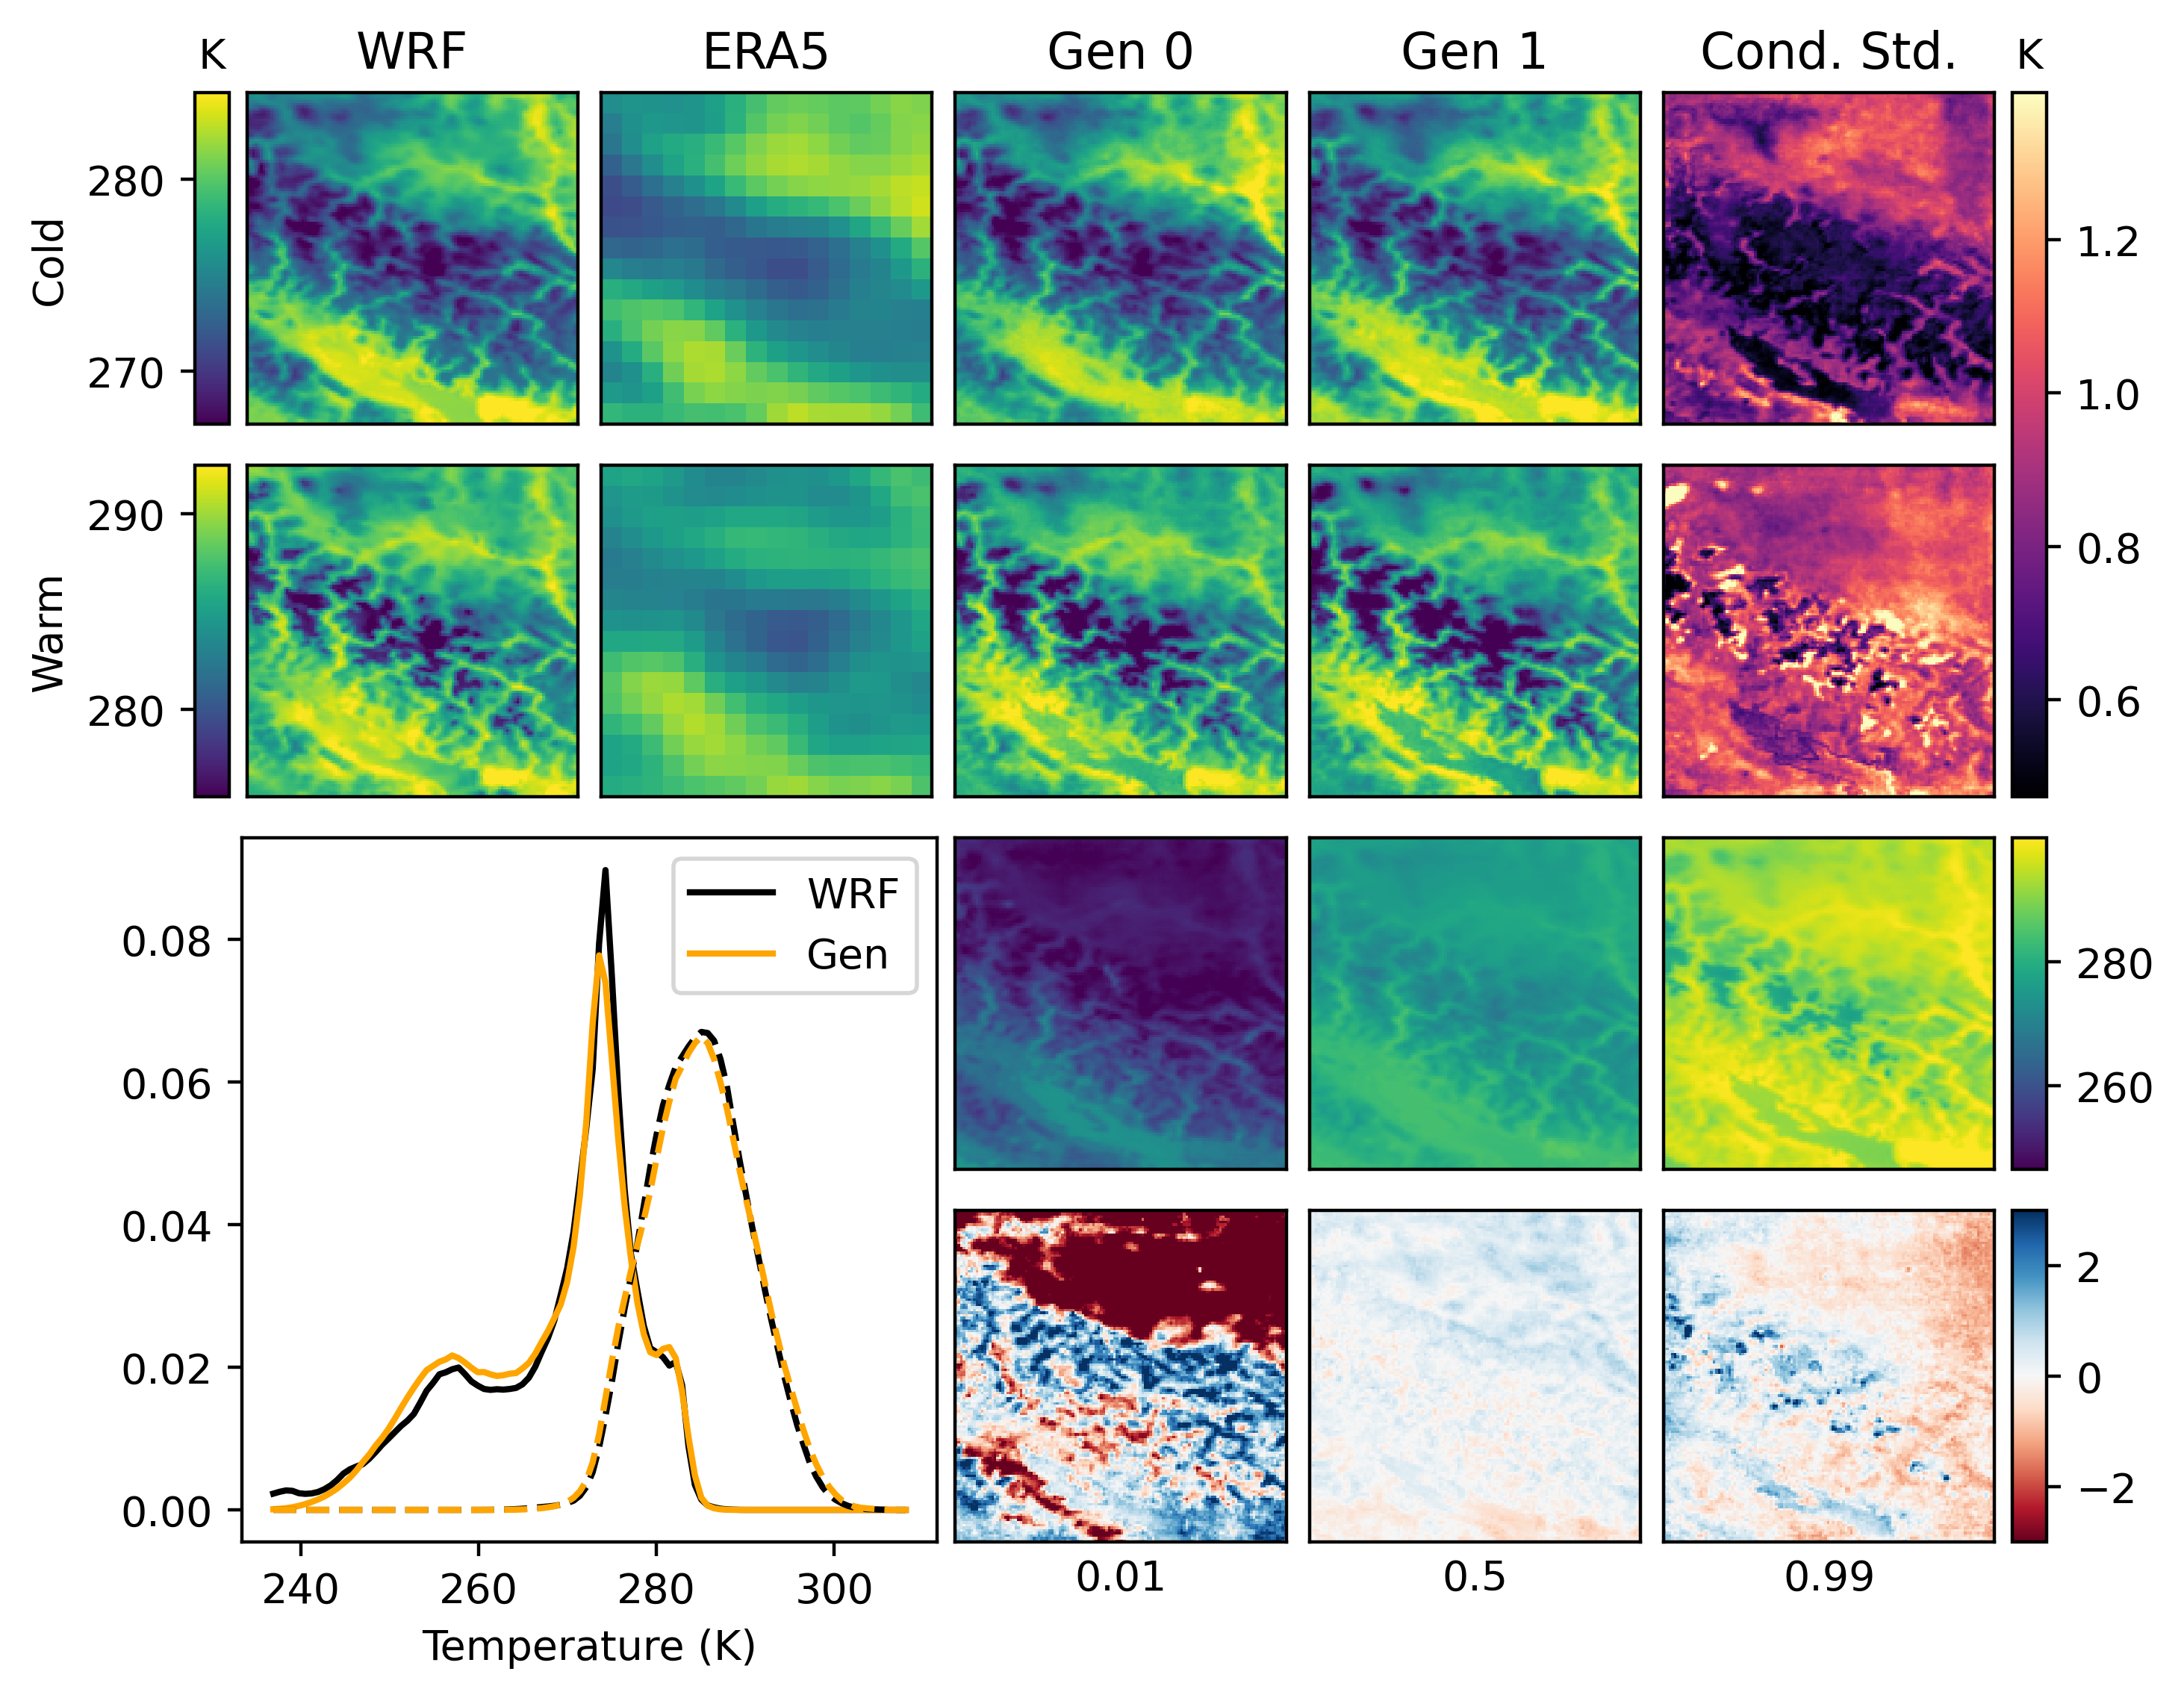
\includegraphics[width=\textwidth,angle=0]{final/Temperature_Fig.png}\\
  \caption{Evaluation of univariate GAN downscaling of temperature for the Southwest study area. Top two rows show respectively an example cold and warm sample, with the WRF field, LR conditioning field (showing the continental outline), two stochastic realisations, and the conditional pixel-wise standard deviations across 100 ensemble members. The third row shows 0.01, 0.5, and 0.9 quantiles over 3000 random samples from the generated fields, and the bottom row shows the corresponding quantile differences (truth - generated). The left-bottom panel shows overall PDFs of pixel values for January samples (solid) and July samples (dashed).}\label{temperature}
\end{figure}

Specific humidity proved to be a more challenging variable to accurately downscale (figure \ref{humidity}). In the dry sample especially, the model substantially underestimated the humidity over the Georgia Straight, and while it did predict higher humidity at lower elevations (e.g., over valleys), these were not as clear as in the WRF fields. In the moist sample, while humidity values across the field matched well with WRF, the spatial patterns in the generated fields were more blurred and sharp gradients were not as well represented. Most realisations of the moist sample showed a dry bias on the Eastern side of the field. Overall, the conditional standard deviation was much lower for the dry sample than the moist sample. The moist sample showed low deviation in the ocean, but relatively high variability in the mountains near the coast. Distributions of pixel values for January and July showed substantially more bias than with temperature, especially for July, where the PDF of generated values shows underdispersion. 

Pixelwise 0.01 quantiles show that the models overestimated humidity through most of the field, except in the Straight of Georgia, where humidity was always underestimated. Median values were similar, but showed a slight underestimation across the field. For 0.99 quantiles (very moist) the models largely underestimated humidity, except on the tops of mountains.
\begin{figure}[H]
  \noindent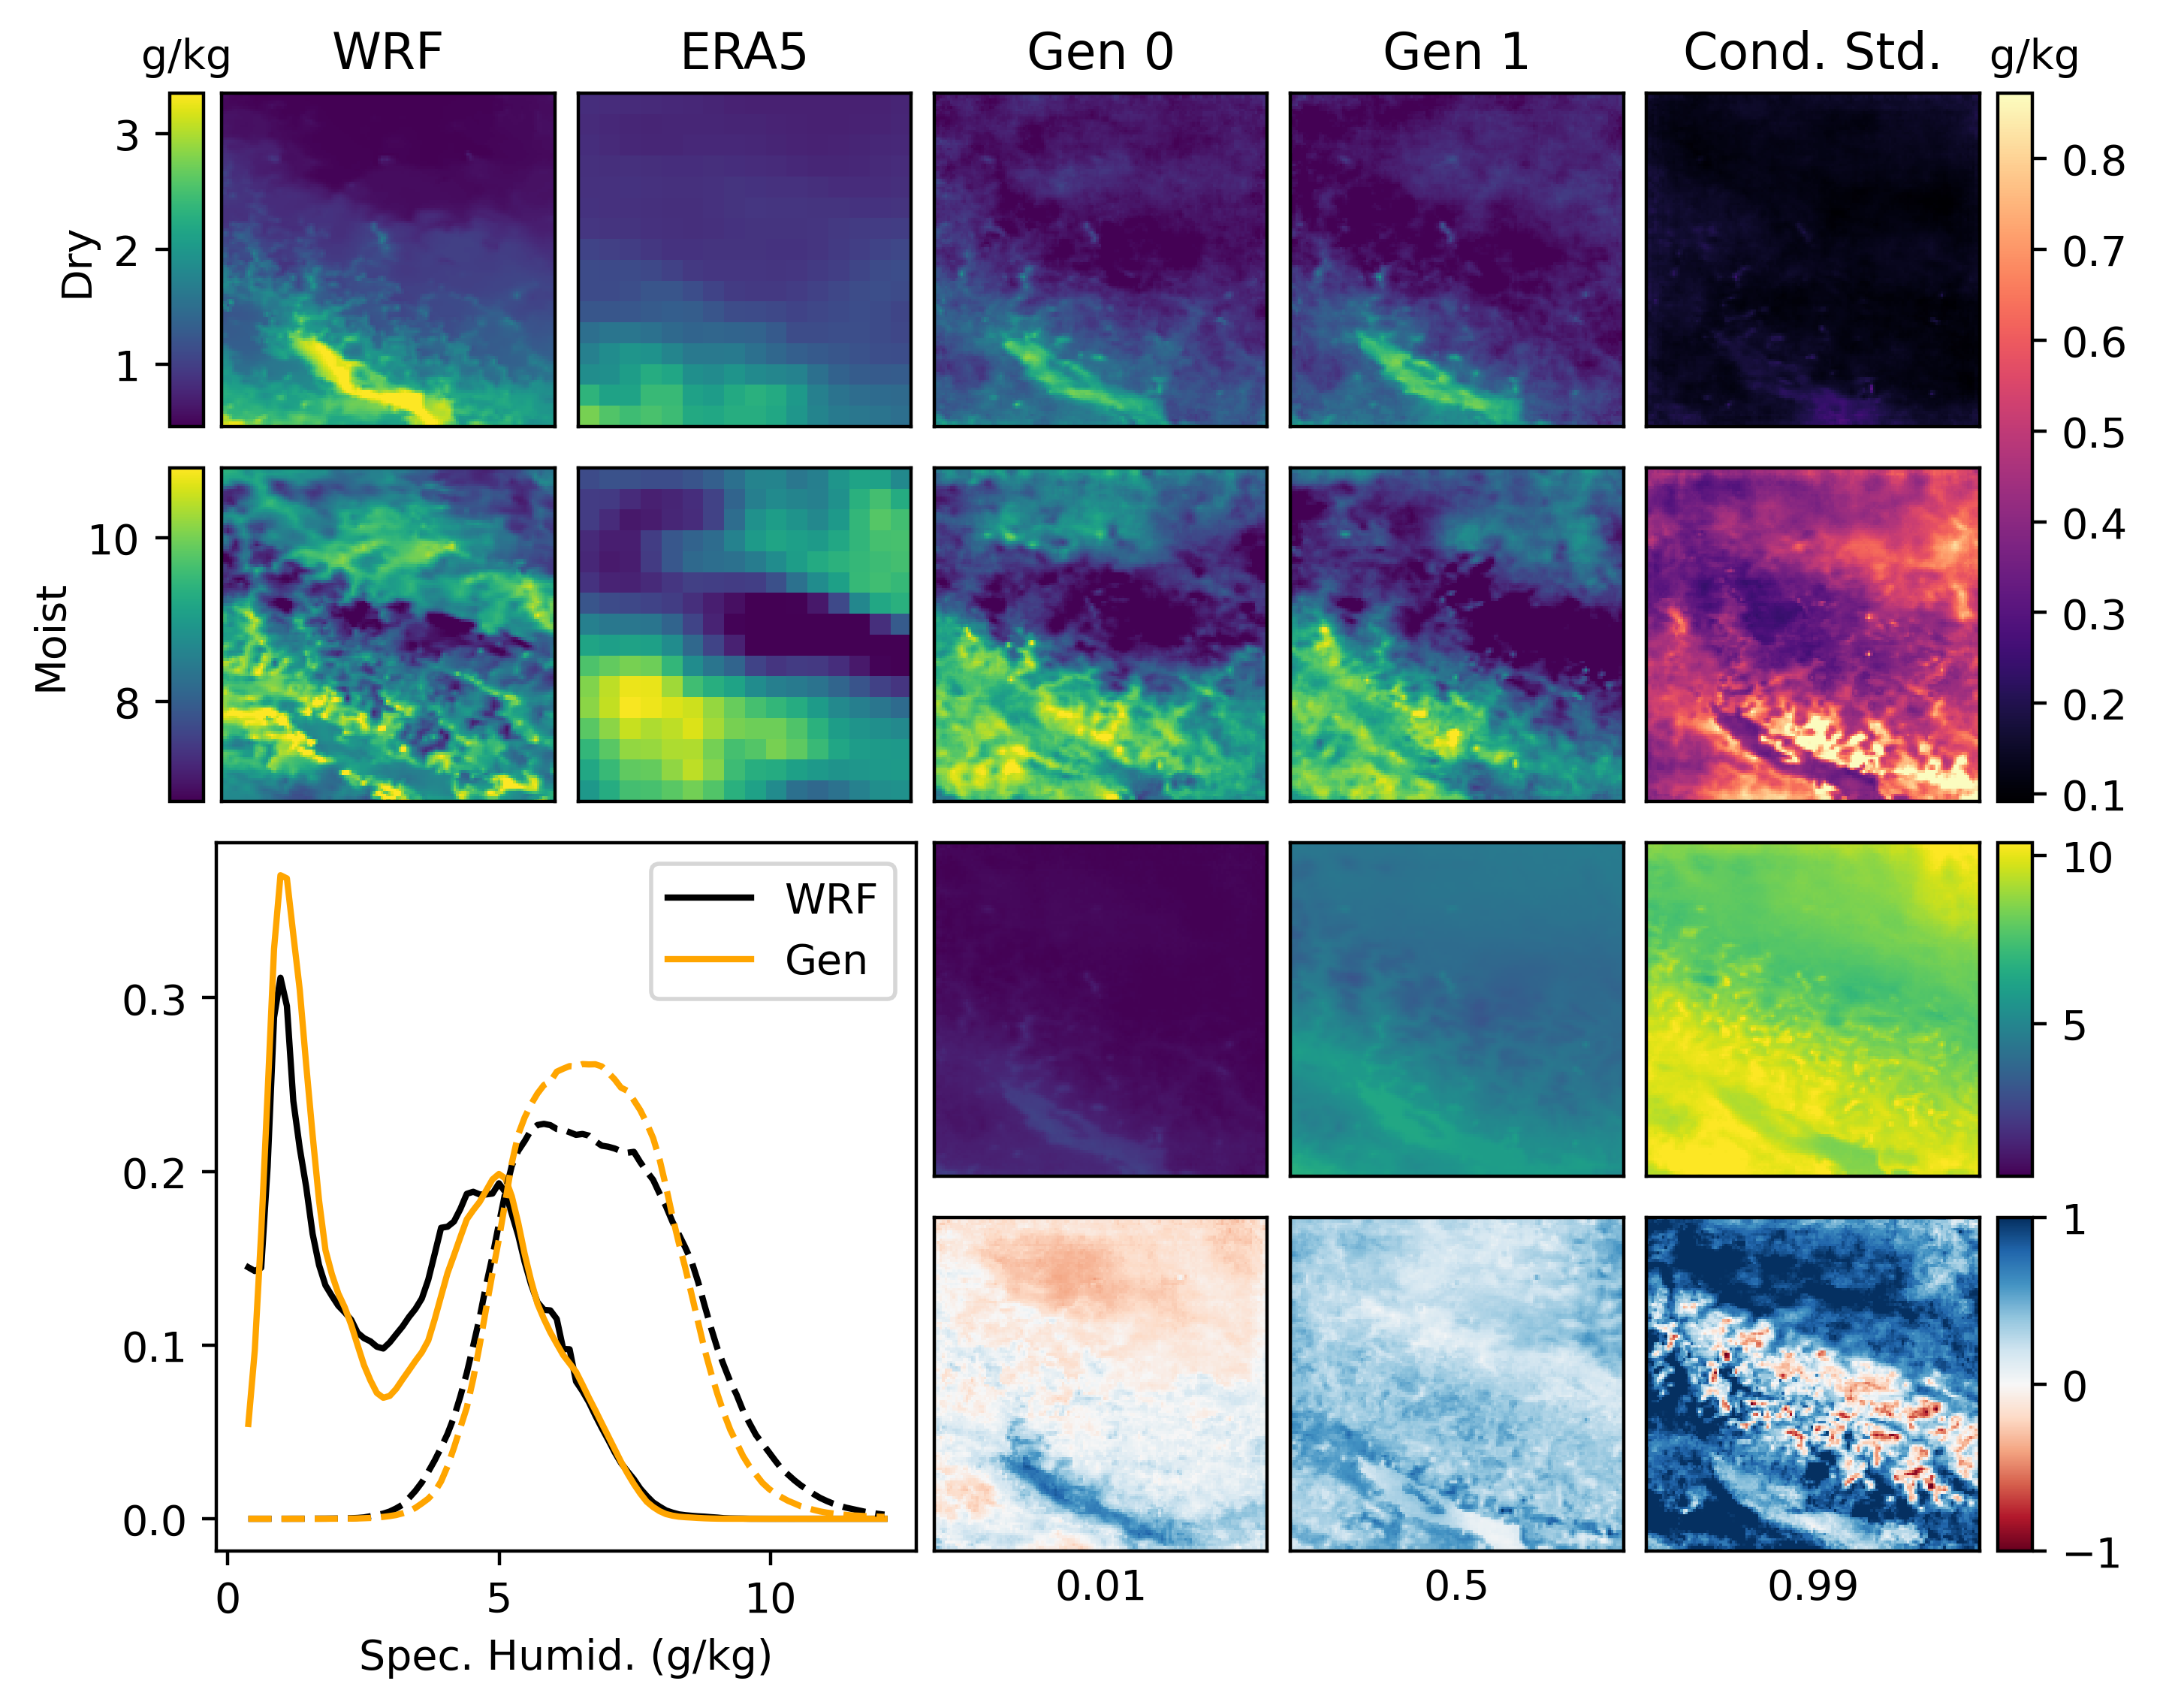
\includegraphics[width=\textwidth,angle=0]{final/Humidity_Fig.png}\\
  \caption{Evaluation of univariate GAN downscaling of specific humidity for the Southwest study area. Top two rows show respectively an example dry and moist sample, with the WRF field, LR conditioning field (showing the continental outline), two stochastic realisations, and the conditional pixel-wise standard deviations across 100 ensemble members. The third row shows 0.01, 0.5, and 0.9 quantiles over 3000 random samples from the generated fields, and the bottom row shows the corresponding quantile differences (truth - generated). The left-bottom panel shows overall PDFs of pixel values for January samples (solid) and July samples (dashed).}\label{humidity}
\end{figure}

The GAN also performed well at downscaling precipitation (figure \ref{precip}). The light-rain-hour sample shows a large degree of variation between realisations, as is desired. The heavy rain sample also shows high conditional standard deviation, although relative to the mean, not as much as the light rain sample. With precipitation especially, it is noticeable that single realisations of the generated fields often show different patterns than the WRF field. However, as our goal is to sample from the distribution of possible downscalings, this is expected. 

Pixel value distributions were very similar in January and July, and were combined in the PDF for better visual interpretation. Generated and WRF distributions matched well, although the GAN slightly underestimated extreme precipitation events. This underestimation of heavy precipitation is also apparent in the pixelwise quantile difference maps, which show good calibration for 0.01 quantiles and medians, but predominantly underestimation of 0.99 quantiles.  
\begin{figure}[H]
  \noindent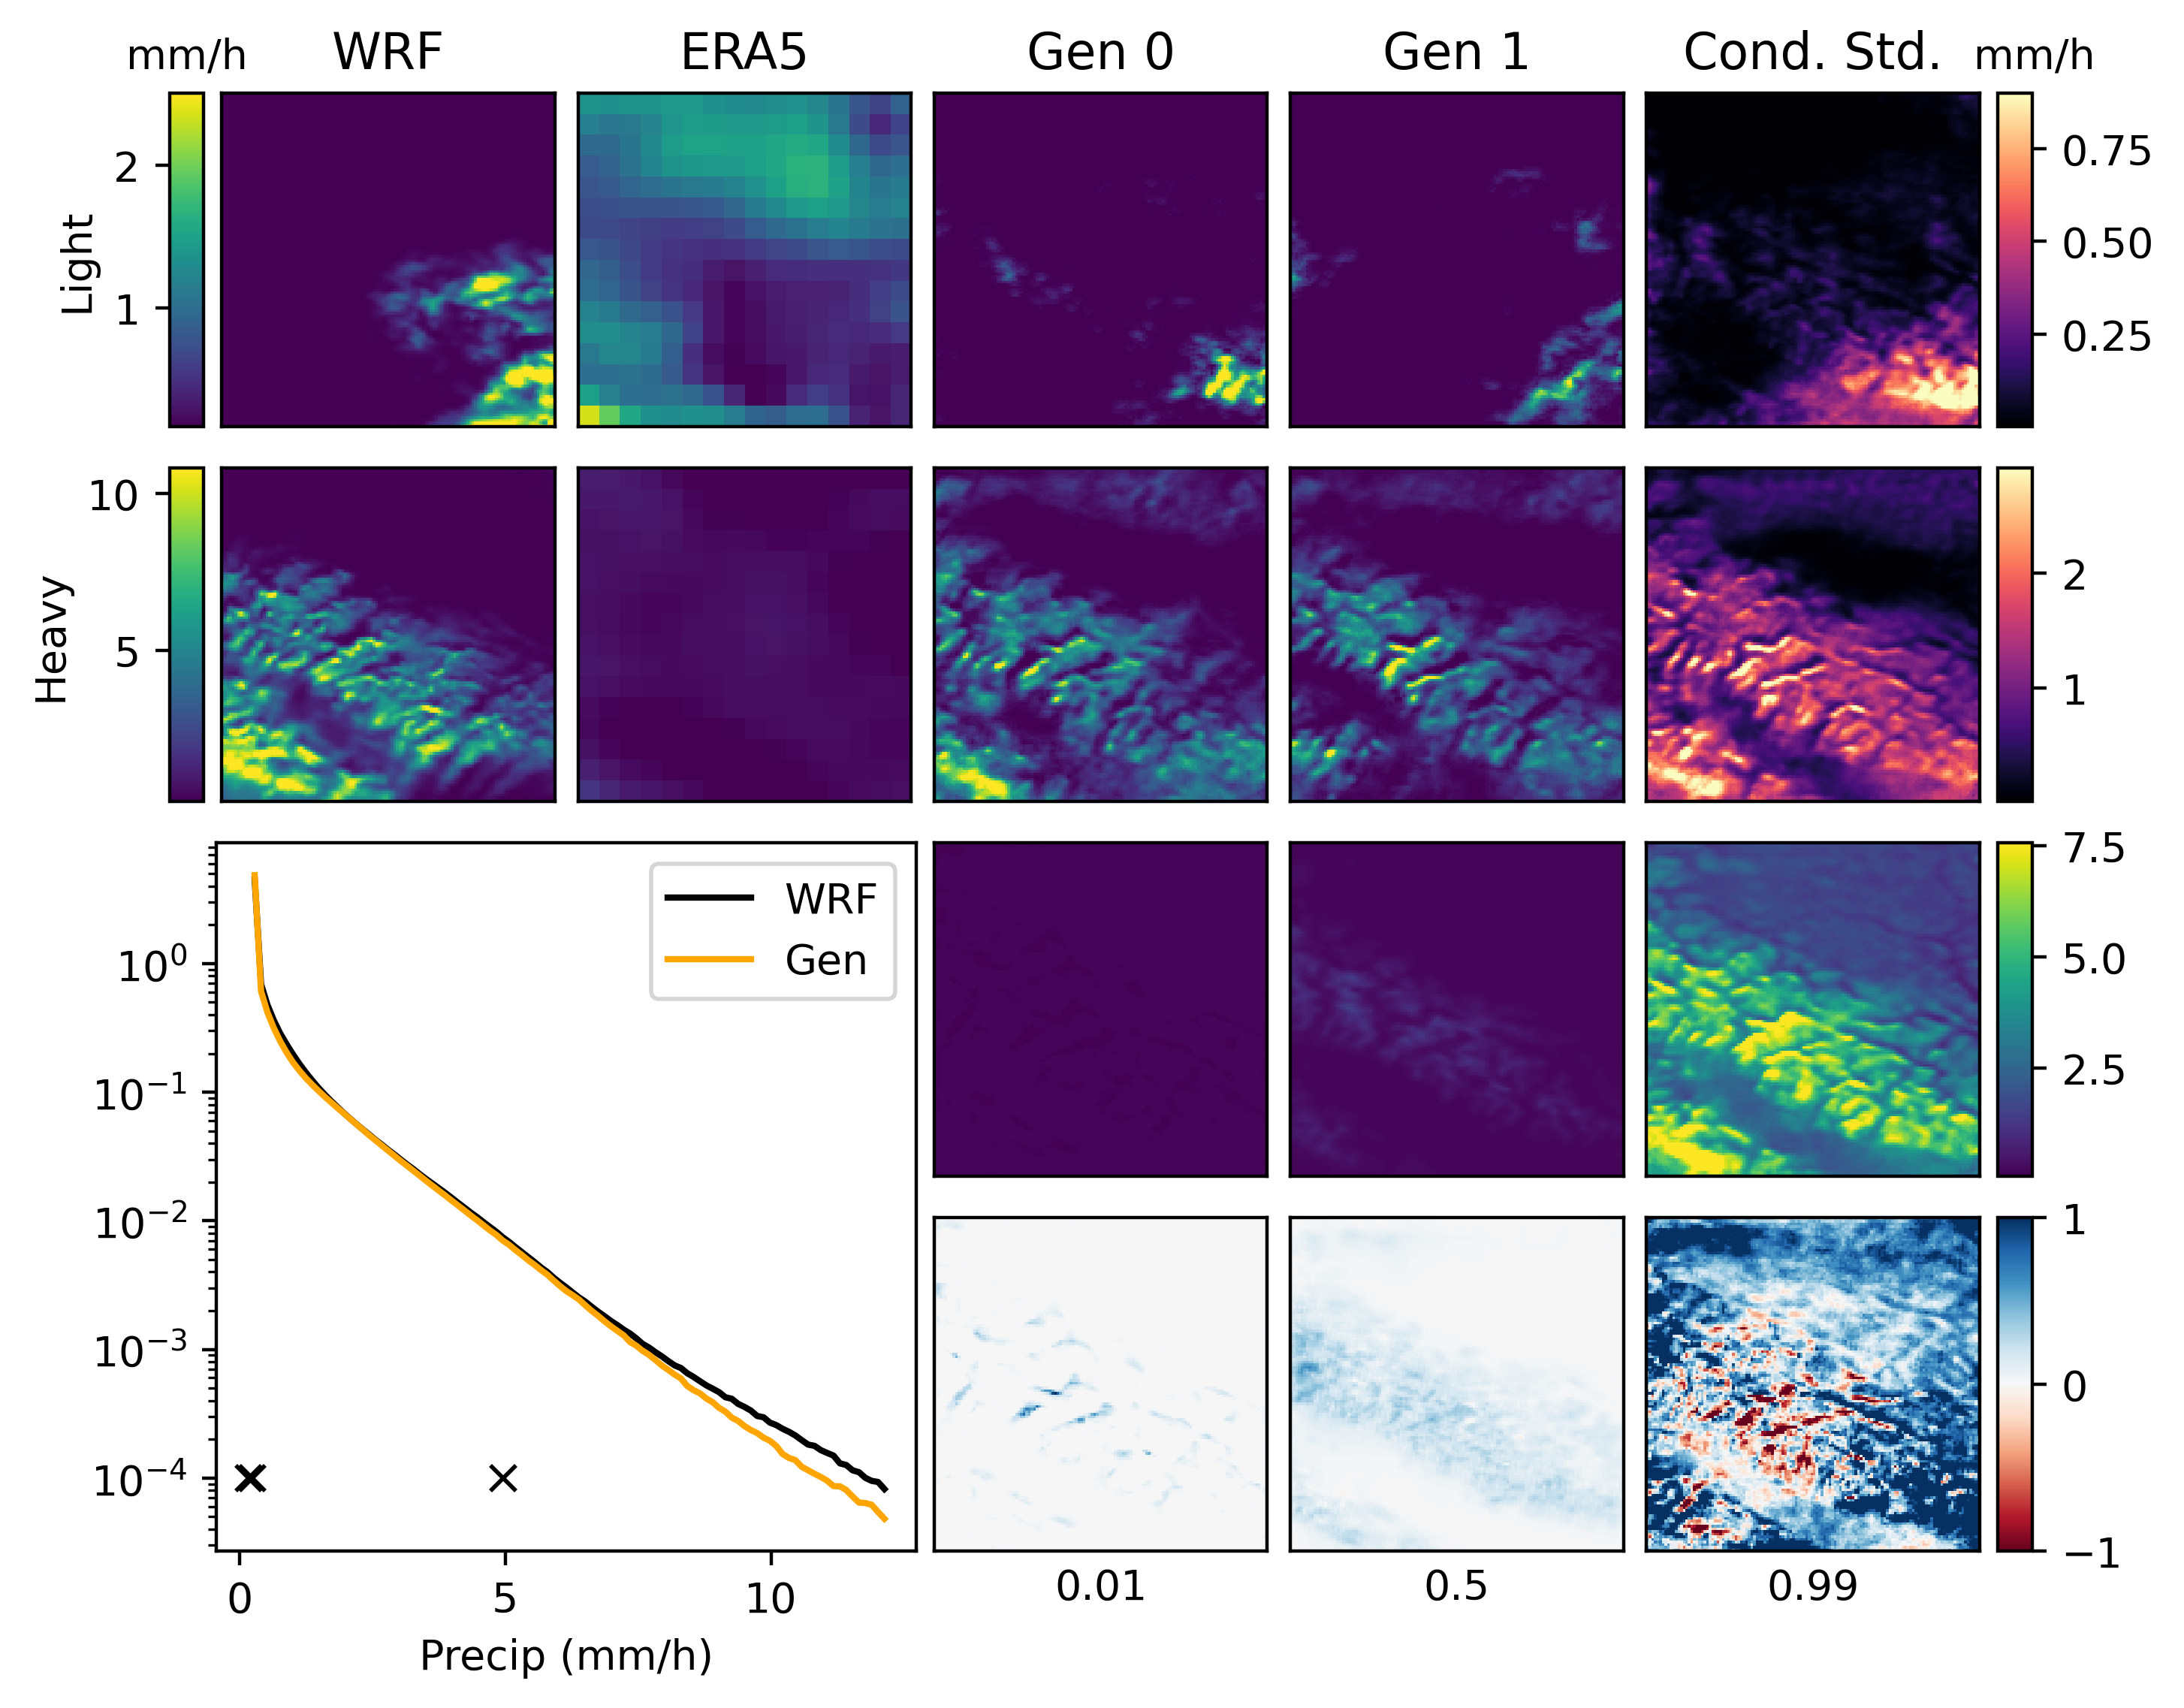
\includegraphics[width=\textwidth,angle=0]{final/Precip_Fig.png}\\
  \caption{Evaluation of univariate GAN downscaling of precipitation for the Southwest study area. Top two rows show respectively an example light rain and heavy rain sample, with the WRF field, LR conditioning field, two stochastic realisations, and the conditional pixel-wise standard deviations across 100 ensemble members. The third row shows 0.01, 0.5, and 0.9 quantiles over 3000 random samples from the generated fields, and the bottom row shows the corresponding quantile differences (truth - generated). The left-bottom panel shows overall PDFs of pixel values for months January to July combined. Crosses indicate the location of 0.01, 0.5, and 0.99 quantiles. All timesteps that had zero precipitation in the WRF field were removed prior to analysis.}\label{precip}
\end{figure}

We found that covariate choice was especially important for precipitation. Initial models, which only included LR precipitation, temperature, evaporation, and pressure produced fuzzy and biased downscaling. Addition of CAPE and wind components substantially improved results. 

Stochastic GANs did a much better job of capturing extreme precipitation than equivalent deterministic models (figure \ref{precipdistr}). While both models slightly underestimated the probability of high precipitation compared to WRF, the stochastic model matched the distribution of the WRF data well, while the deterministic model did not predict any precipitation values $<$ 18 mm/h. Both models show a low-precipitation bias for light precipitation ($<$ 2.5 mm/h).
\begin{figure}[H]
  \noindent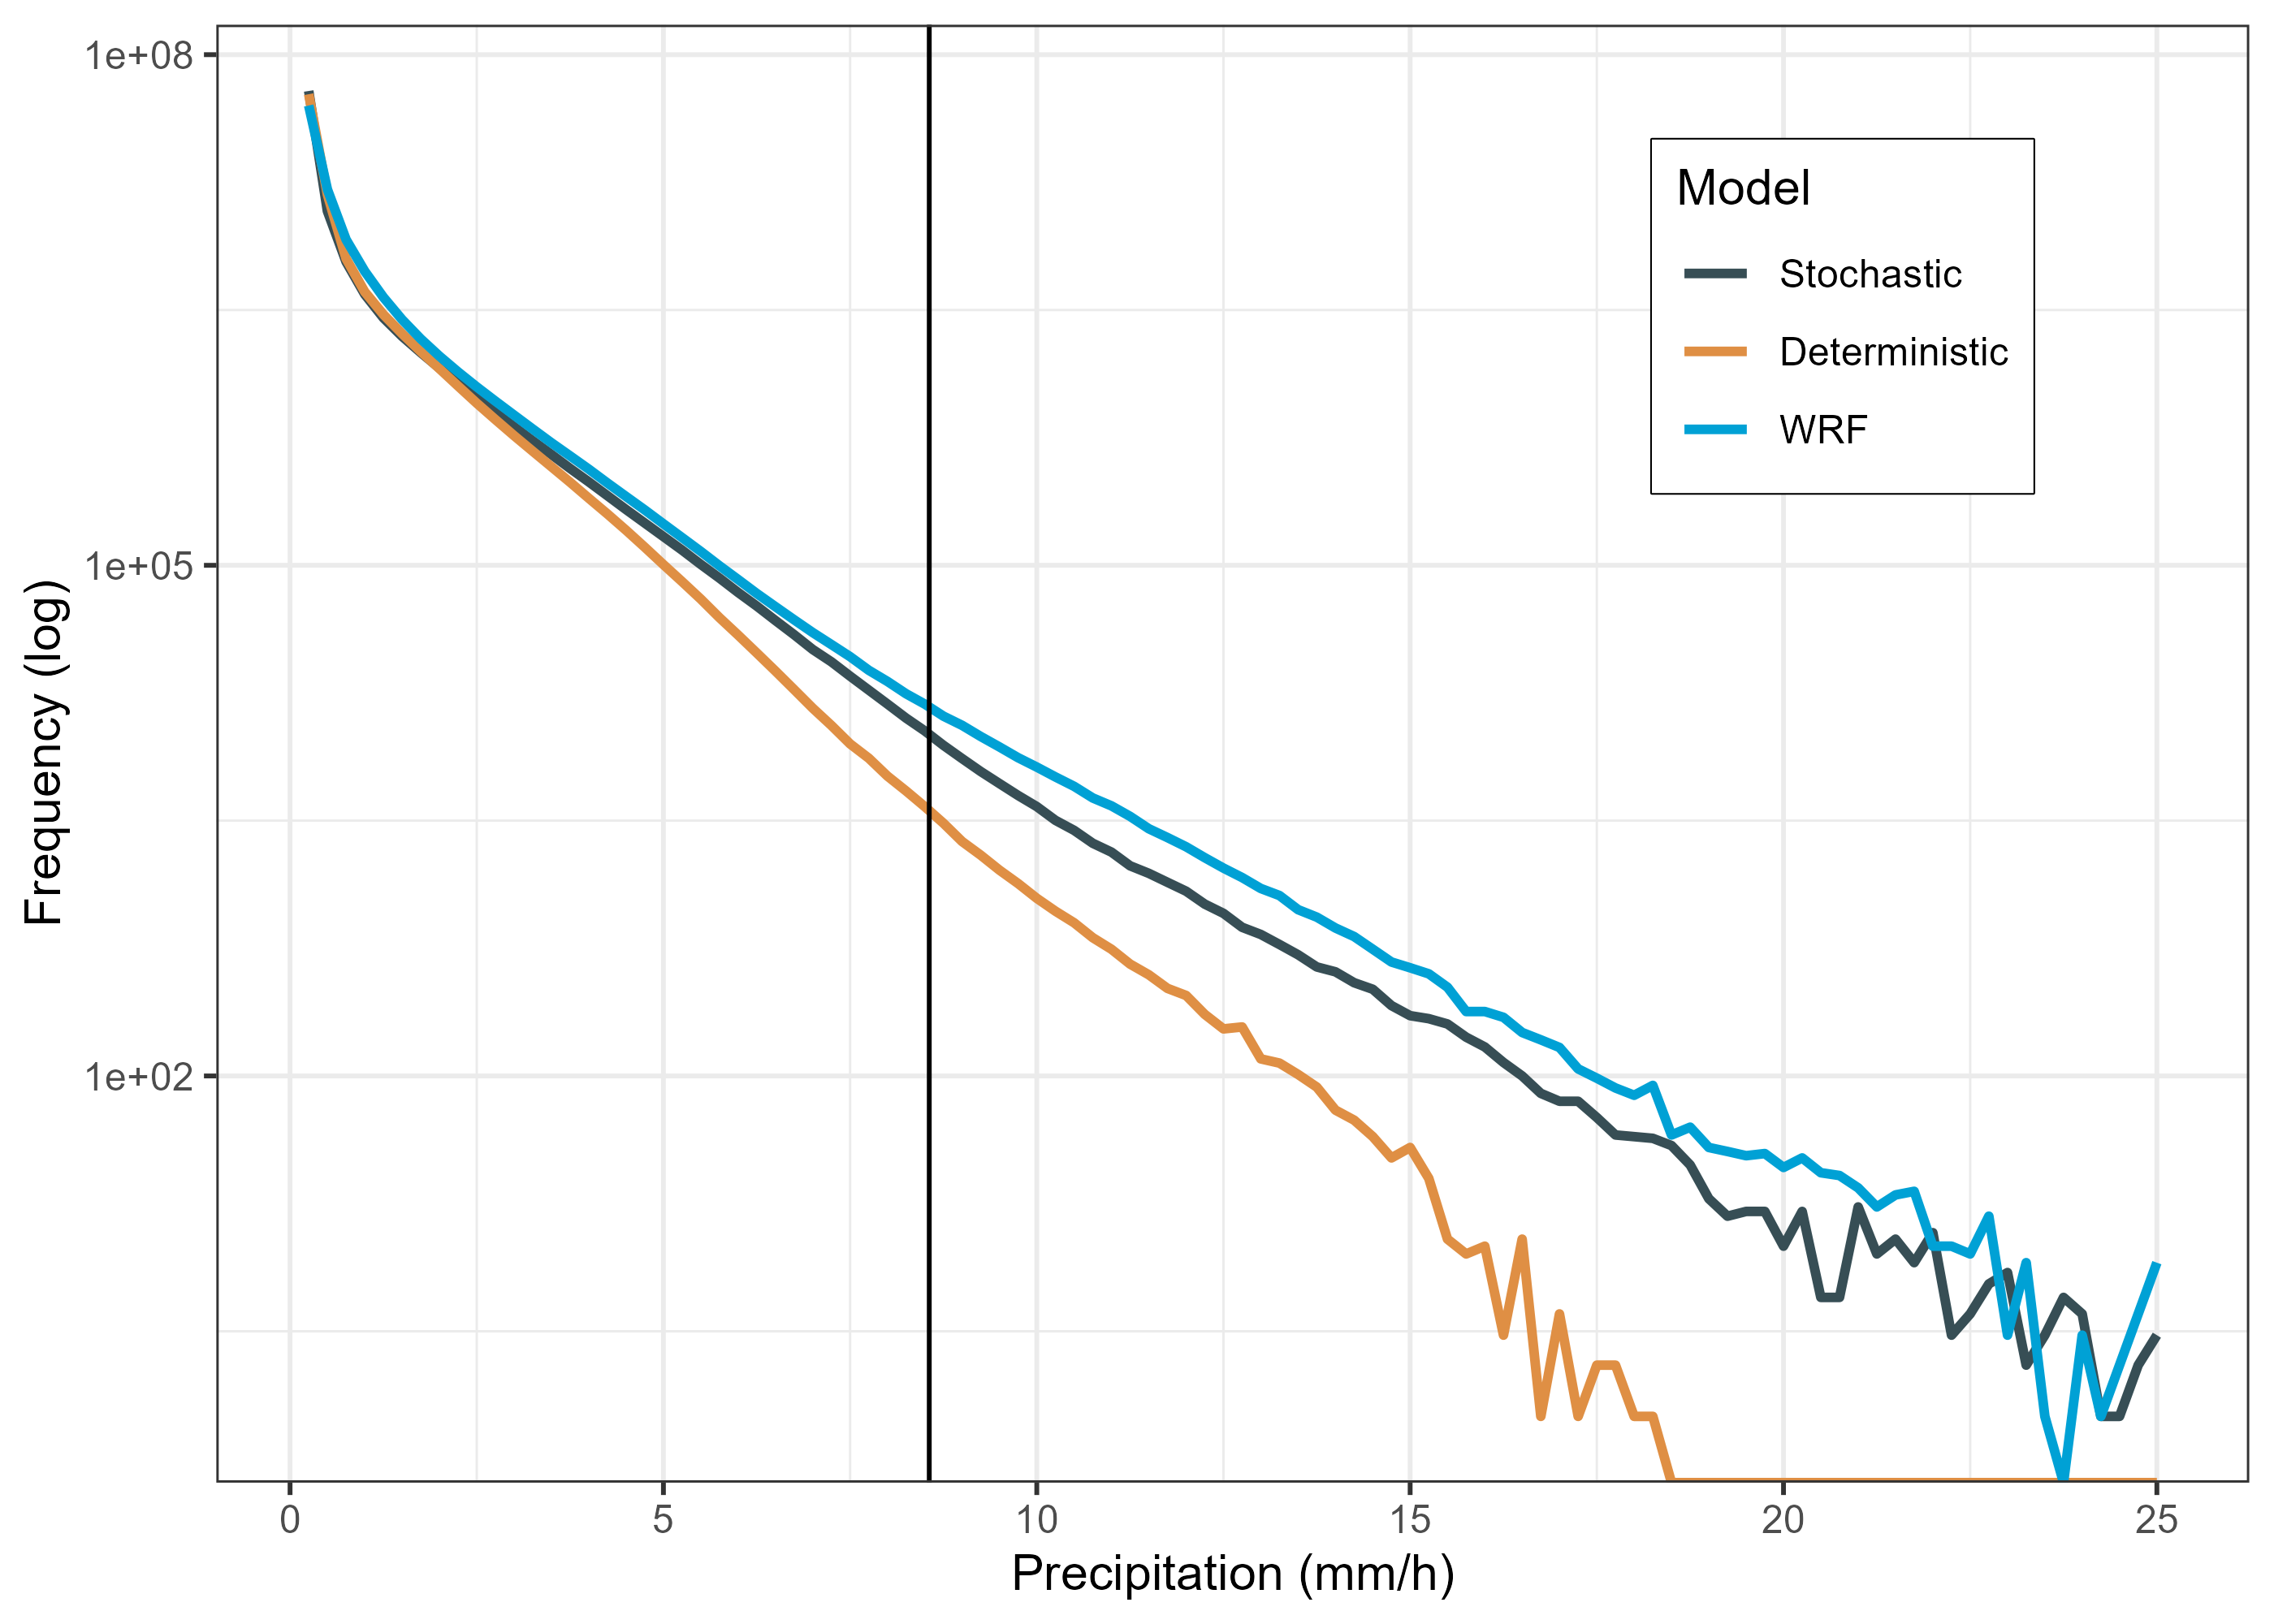
\includegraphics[width=0.5\textwidth,angle=0]{final/Precip_Distr.png}\\
  \caption{Distributions of pixel values for precipitation fields, comparing WRF, deterministic generated, and stochastic generated. Distributions were estimated from all pixels of one year of hourly samples. Note the y-axis is shown on a log scale. }\label{precipdistr}
\end{figure}
All three variables showed good stochastic calibration and similar spectral power to WRF fields (figure \ref{rasp1}). Median RASP estimates for generated fields showed more than 80\% similarity to corresponding WRF estimates for temperature and humidity. Precipitation also showed good calibration through most of the field, but had a high-power bias at high wavenumbers, corresponding to an overabundance of very fine-scale textures (figure \ref{rasp1}). Precipitation also displayed much more variability between samples that temperature or humidity. This is expected, as precipitation fields vary more across samples than do the other variables. 

\begin{figure}[H]
  \noindent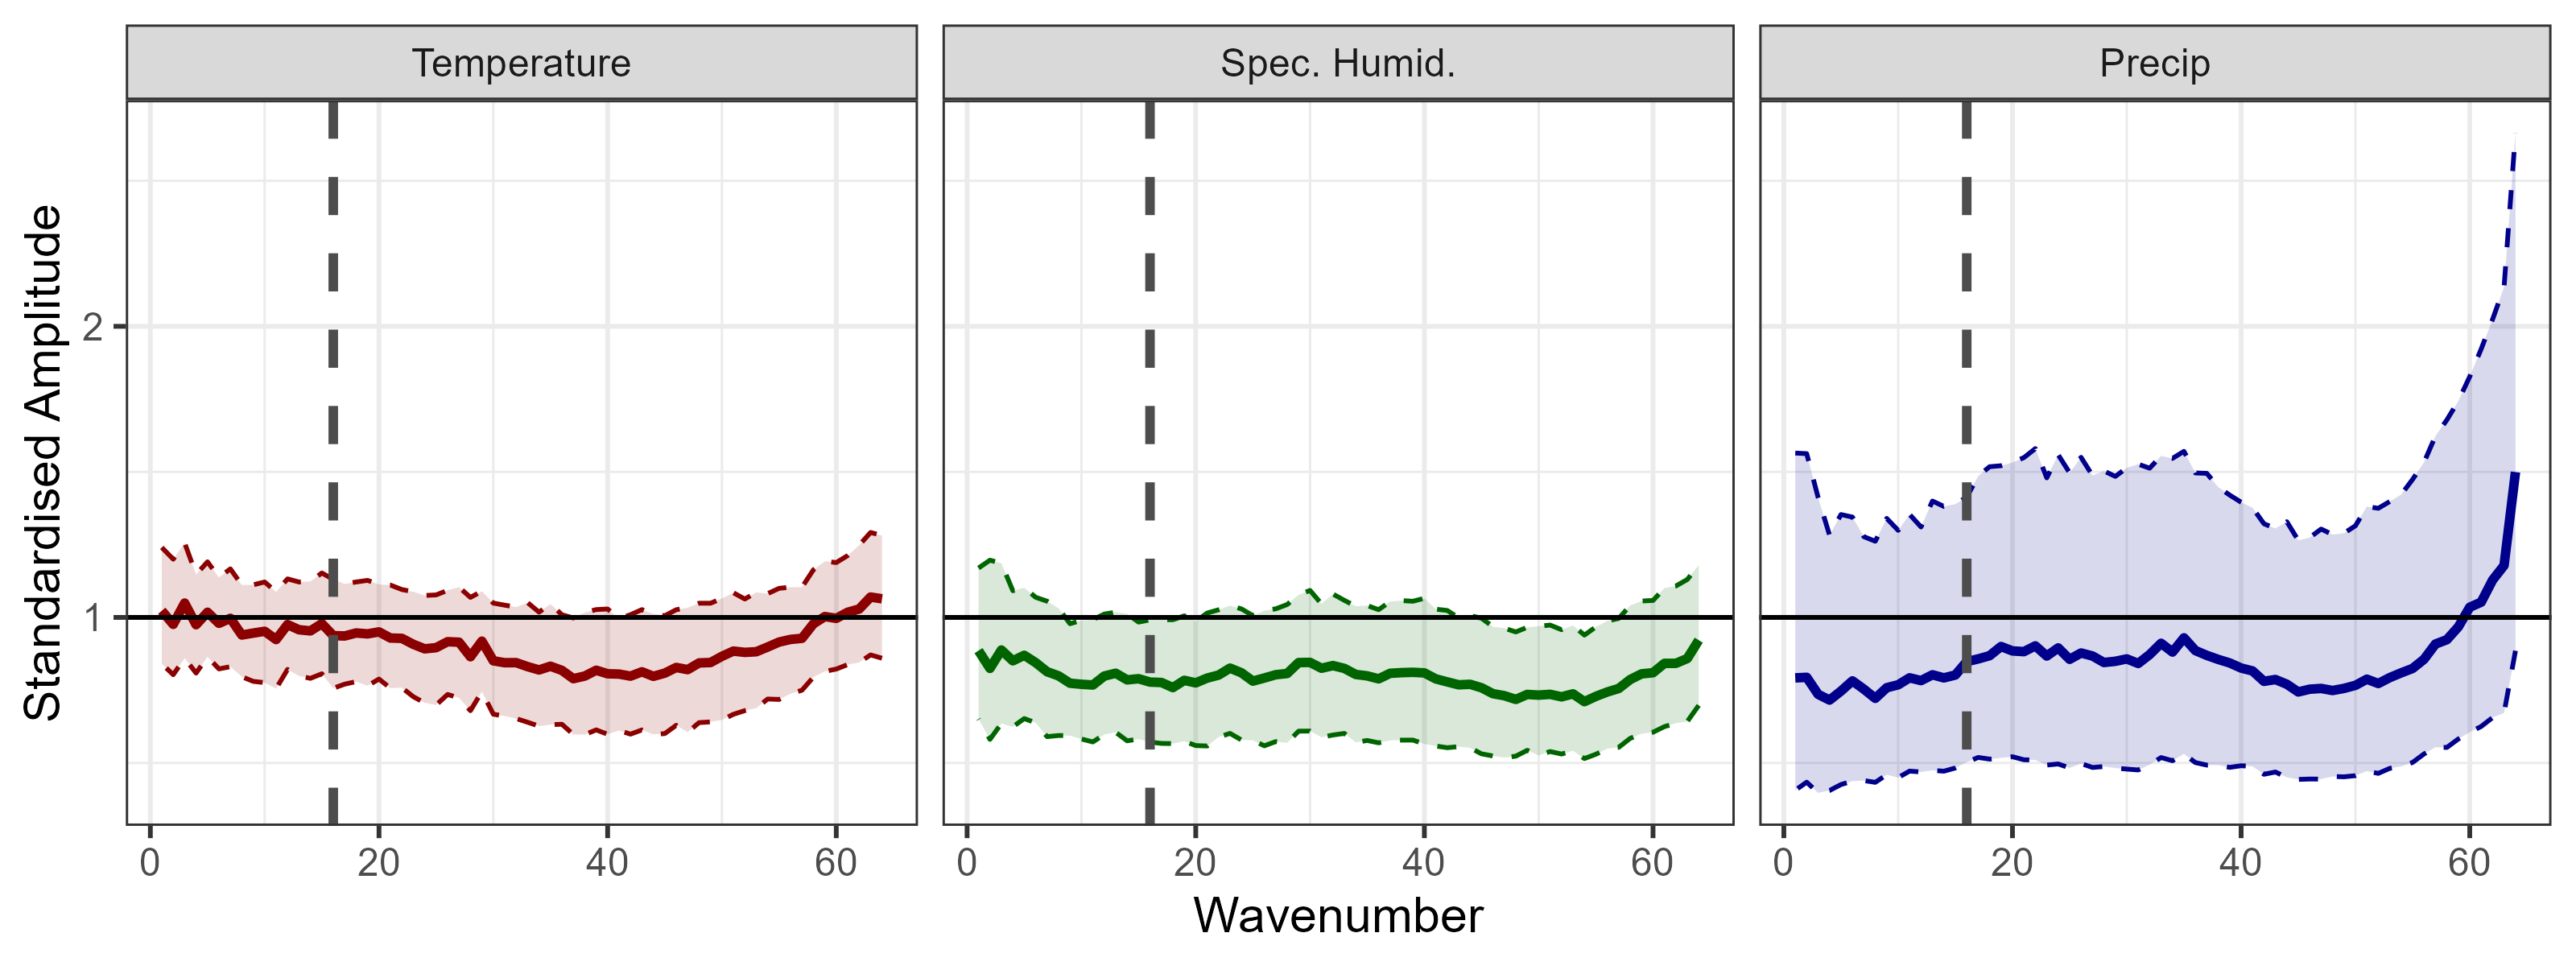
\includegraphics[width=\textwidth,angle=0]{final/RASP_loc1.png}\\
  \caption{RASP metric for the three variables. Spectral powers are standardised to ground truth fields, and metrics are calculated across 1200 randomly selected fields. Solid lines show median spectral power, shaded region show inter-quartile range.}\label{rasp1}
\end{figure}

Considering calibration of conditional distributions for individual samples, all variables showed slight underdispersion, with ranks concentrated at either end of the scale (figure \ref{rankhist1}a) instead of being uniformly distributed across possible ranks. Temperature showed good calibration for the median and 0.99 quantile sample, but underestimation over most of the range for the 0.01 quantile sample. Specific humidity showed the most consistent underdispersion, especially in the 0.01 and median samples. Precipitation generally was better calibrated, but showed some underestimation in high-precipitation areas. These results also match the rank histogram across timesteps; temperature and humidity both showed slight underdispersion of conditional distributions, and precipitation showed underestimation of high values (figure \ref{rankhist1}b).  
\begin{figure}[H]
  \noindent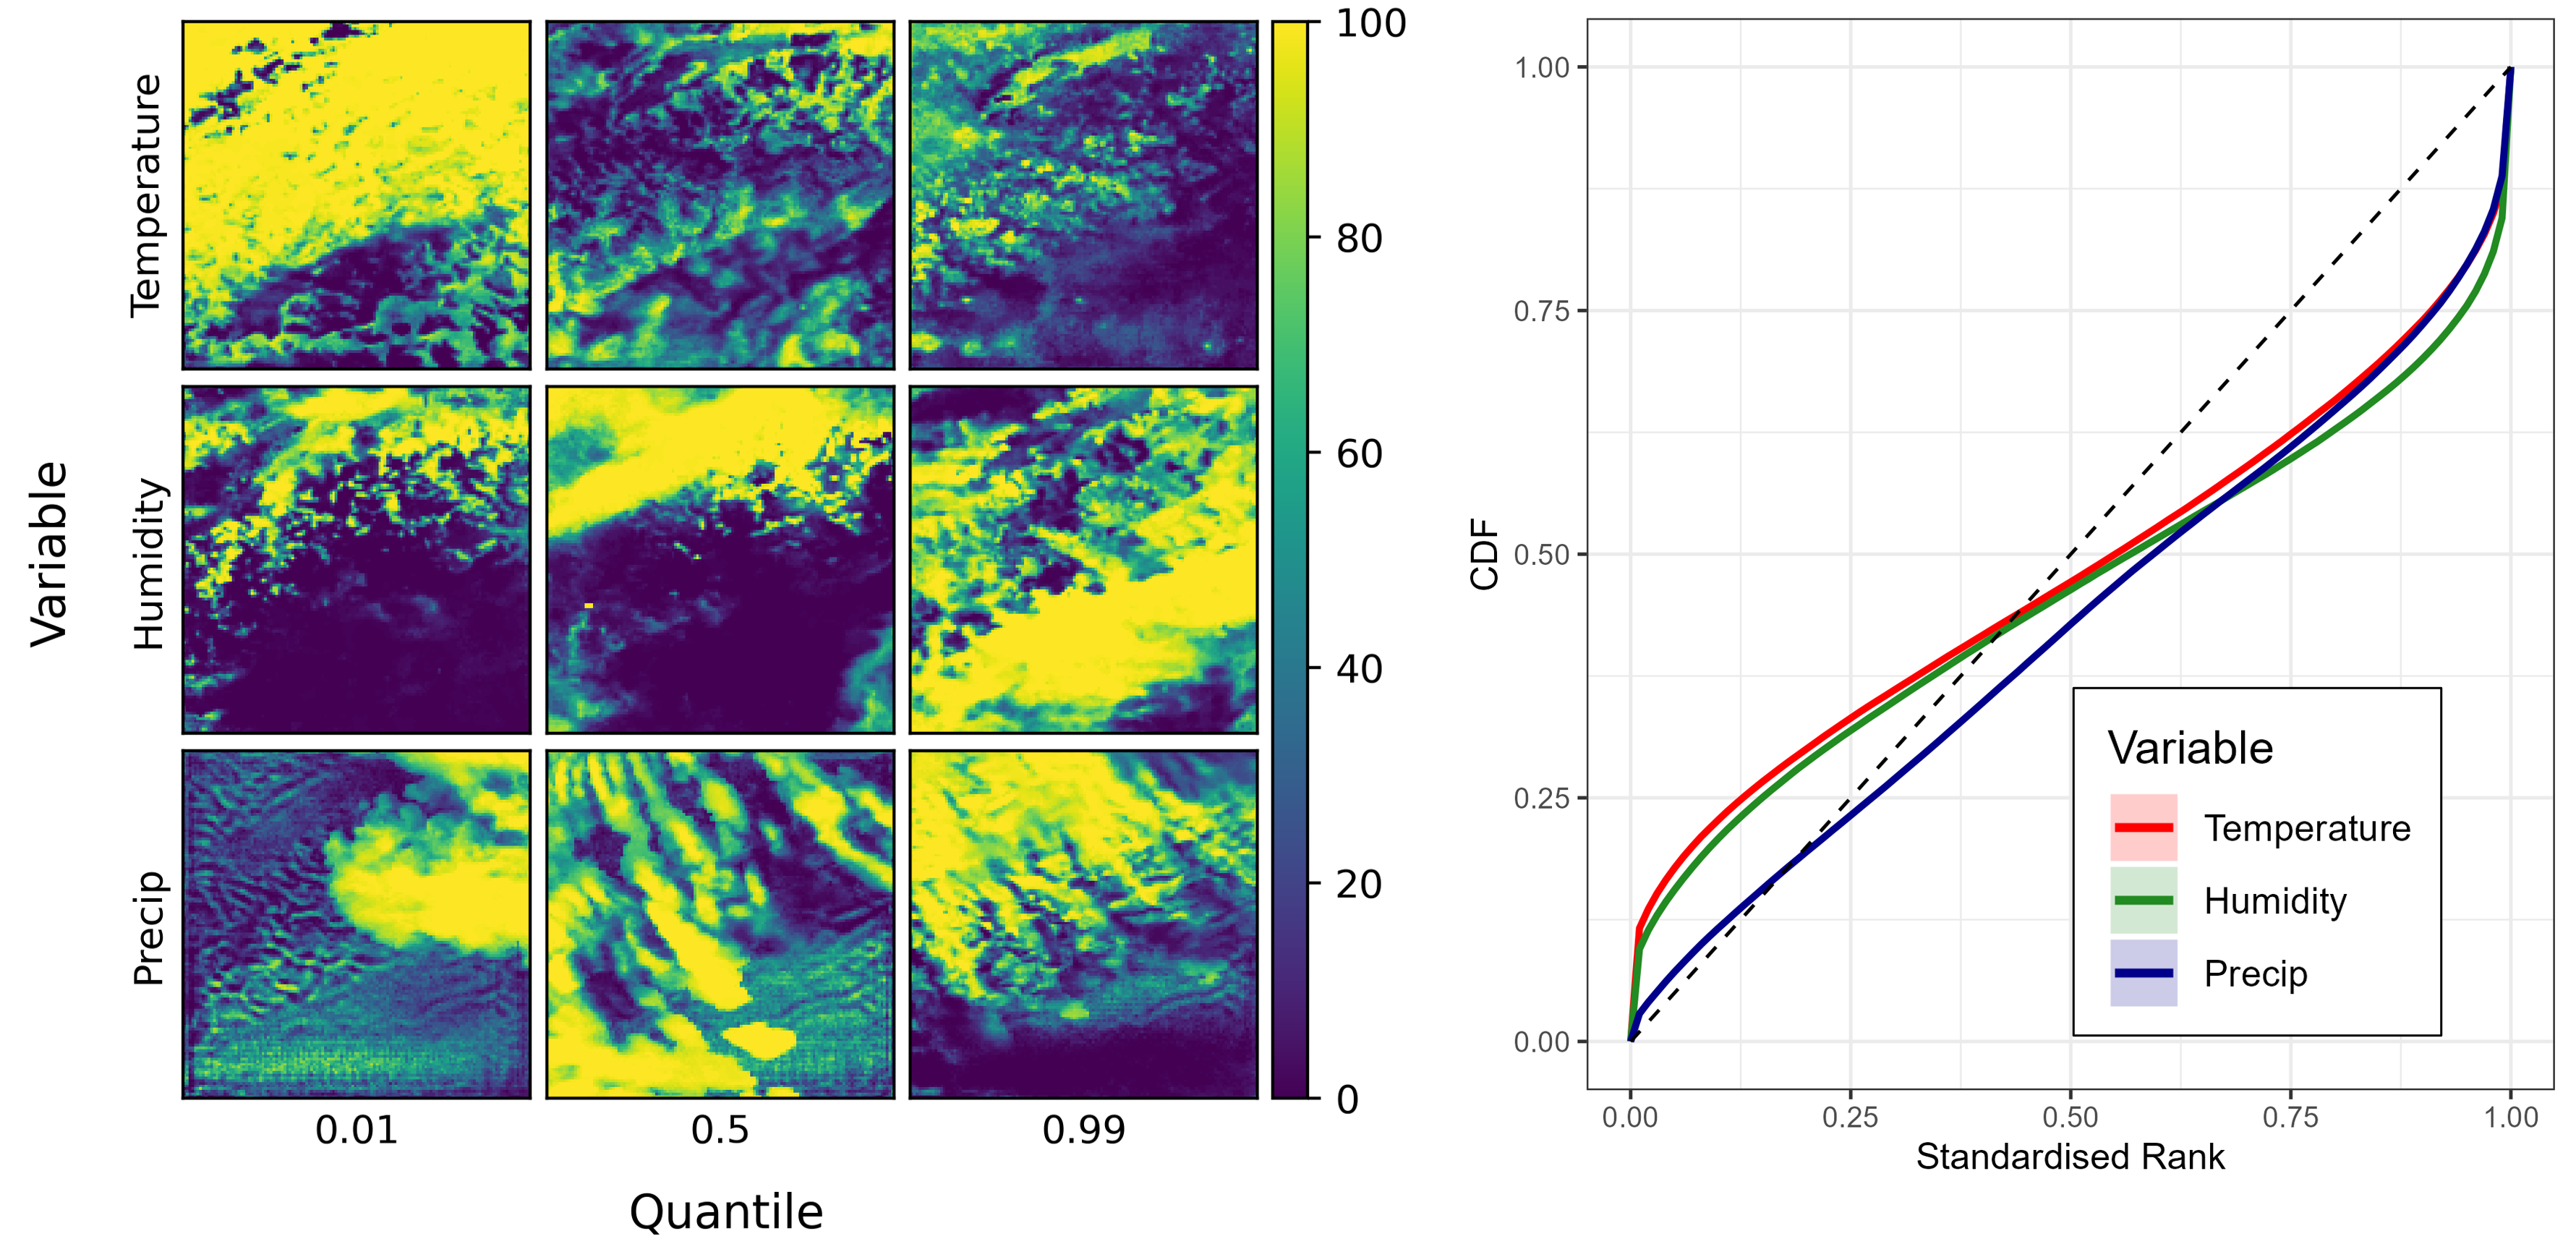
\includegraphics[width=\textwidth,angle=0]{final/Loc1_RankHist.png}\\
  \caption{a) Rank histogram maps for individual samples showing, for each pixel, the rank of the WRF pixel compared to an ensemble of 100 realisations. b) CDF of rank histograms showing stochastic calibration of conditional distributions for univariate models of temperature, specific humidity, and precipitation. Rank histograms were calculated across 100 randomly selected conditioning fields, with 100 HR realisations of each. Dashed line shows reference uniform CDF.}\label{rankhist1}
\end{figure}

\subsection{Multivariate Prediction}

Multivariate GANs showed improved dependence structures between pairs of downscaled variables (table \ref{tab:my_table}). Particularly for temperature and humidity, variables from the univariate model had much lower mutual information scores than from the WRF variables, indicating less dependence between variables. Multivariate mutual information scores were mostly slightly lower but close to WRF scores. Temperature and precipitation was the only pair of variables where the multivariate model showed too much dependence - i.e., mutual information scores were higher than for the corresponding WRF variables.  
\begin{table}[ht]
\centering
\caption{Mutual information score between pairs of variables for multivariate prediction, univariate prediction, and WRF. Scores were calculated for each of 600 randomly selected timesteps and averaged. }
\label{tab:my_table}
\begin{tabular}{llrrr}
  \hline
  Variable 1& Variable 2& Multivariate& Univariate& WRF \\ 
  \hline
 Temp & Precip & 0.222 & 0.177 & 0.187 \\ 
   Humid & Precip & 0.198 & 0.177 & 0.210 \\ 
   Humid & Temp & 0.943 & 0.602 & 1.020 \\ 
   \hline
\end{tabular}
\end{table}

While measure of dependence generally improved, marginal statistics for individual variables were worse with the full multivariate model. For temperature, humidity, and precipitation, marginal statistics generated from the full multivariate model were blurrier than those from univariate models (figure \ref{mv_quantiles}). Humidity showed the most severe challenges, missing a lot of fine-scale details. Precipitation, while capturing the general patterns of the marginal statistics, did not capture the high-precipitation values with the multivariate model. 

To asses whether these challenges were due to the inclusion of precipitation, which has substantially different spatial dependence structures, we tested a multivariate model without precipitation. This model showed improved quality, but resulting downscalings were still blurrier than those from the univariate model. This was especially obvious for humidity, which also contained traces of the convolutional filter in both multivariate models.  
\begin{figure}[H]
  \noindent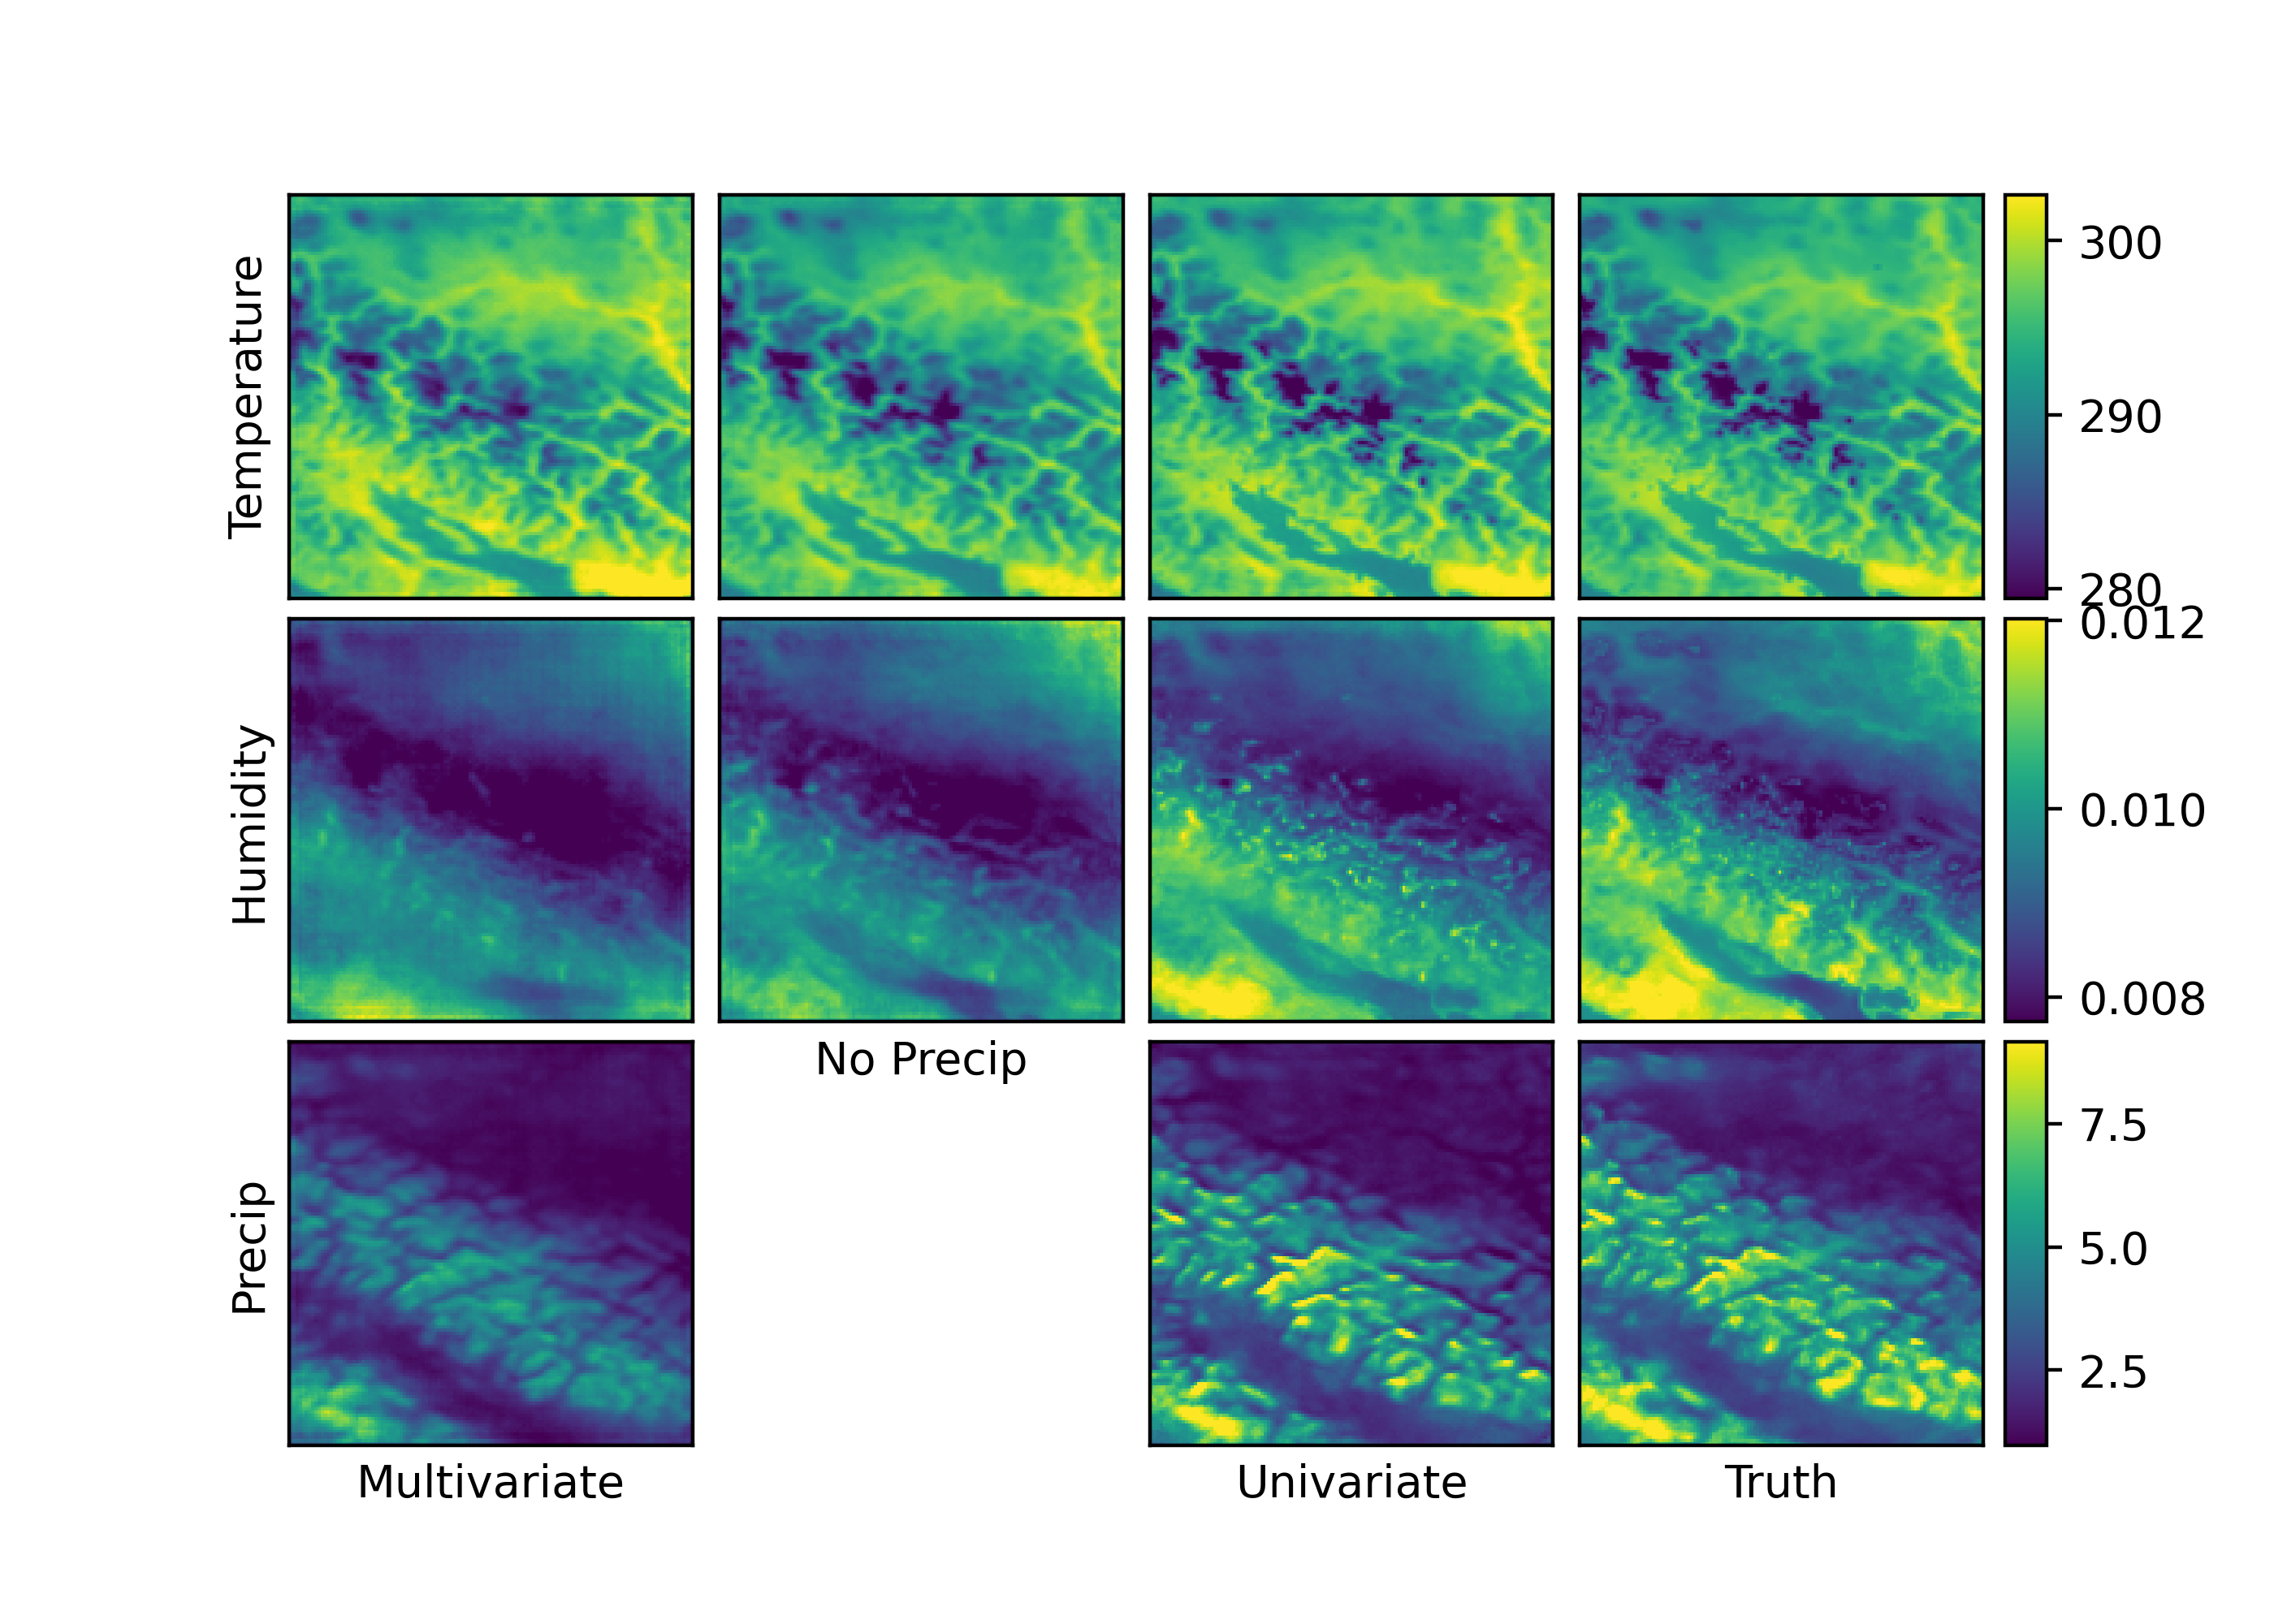
\includegraphics[width=\textwidth,angle=0]{final/MV_UV_Quantiles.png}\\
  \caption{0.99 quantiles for generated temperature, specific humidity, and precipitation fields, using full multivariate prediction, multivariate prediction without precipitation, and univariate prediction. Quantiles were calculated using 3000 randomly selected timesteps. }\label{mv_quantiles}
\end{figure}

Power spectra of all variables showed more bias for multivariate models compared to univariate models, with the NoPrecip model in between (figure \ref{mv_rasp}). Precipitation showed a substantial low-power bias across most wavenumbers in the full multivariate model, often capturing only 25\% of expected power. Humidity and temperature showed large high-power biases at high wavenumbers in both multivariate models, although to a lesser degree in the NoPrecip model, corresponding to the blurriness observed in figure \ref{mv_quantiles}. Both multivariate models also showed a spike in power at wavenumber 32, corresponding to the size of the convolutional filters. Both zonal and meridional wind components showed low-power biases throughout most wavenumbers in the full multivariate model, and high-power biases at high wavenumbers. 
\begin{figure}[H]
  \noindent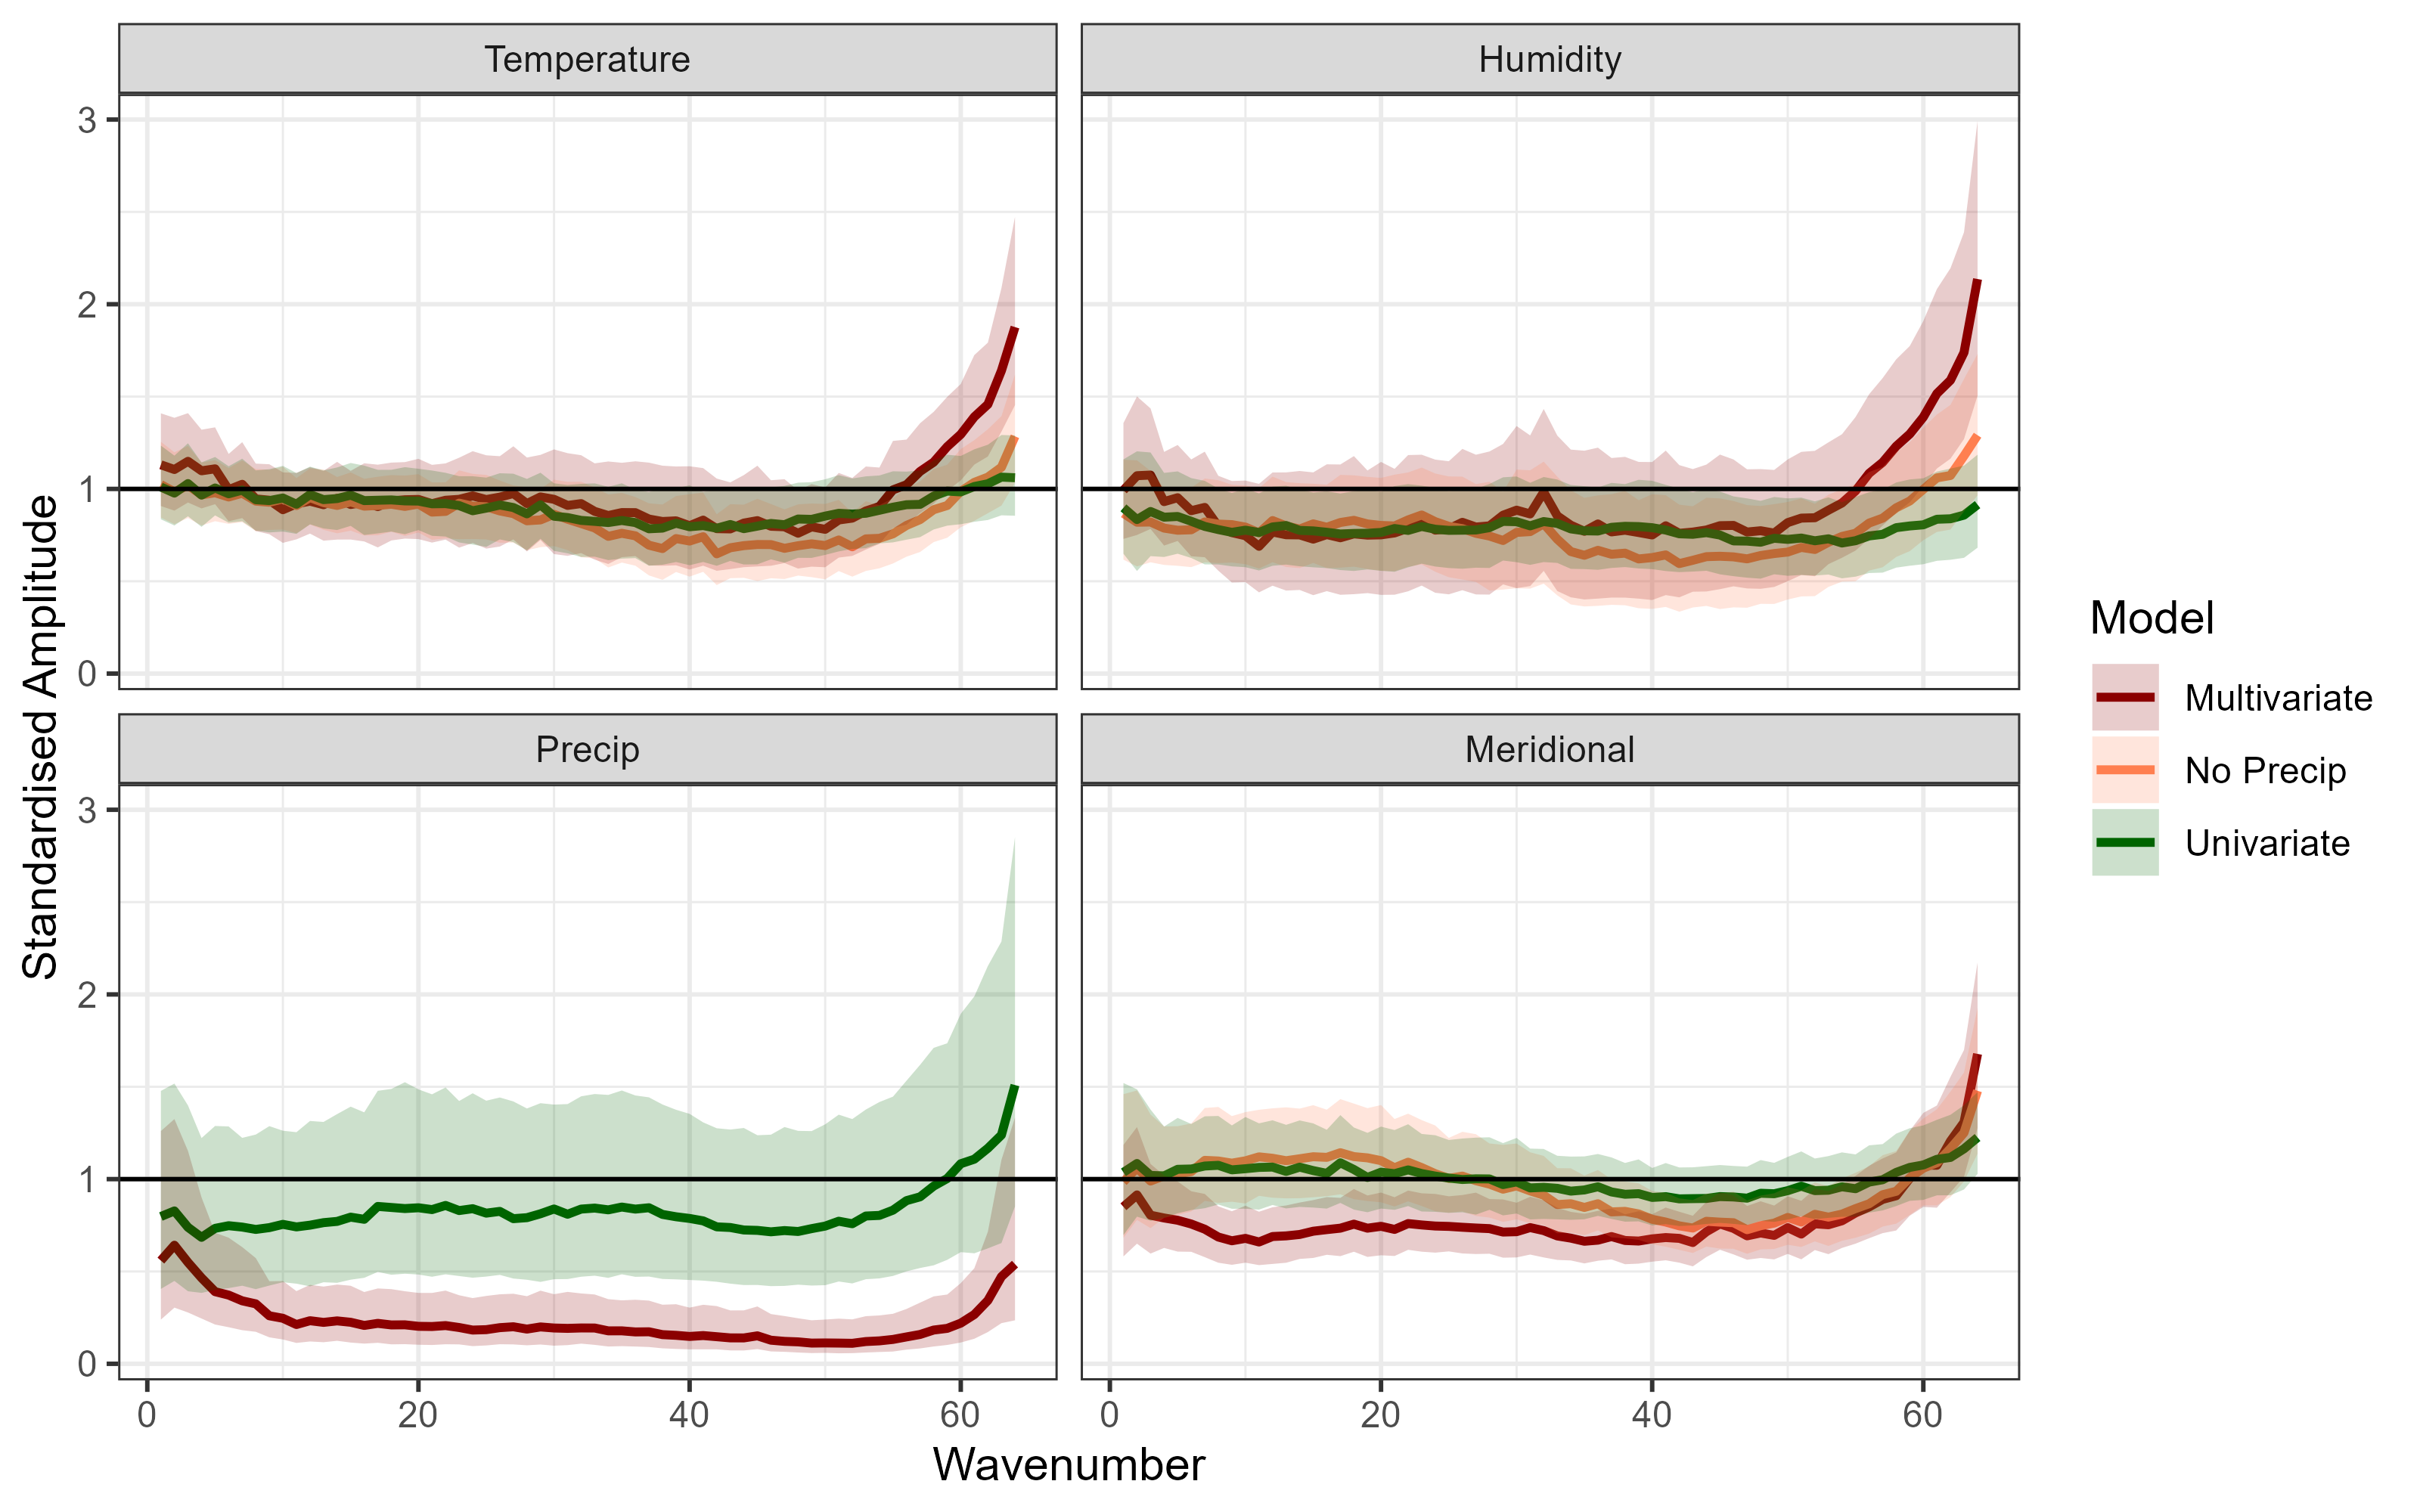
\includegraphics[width=\textwidth,angle=0]{final/MV_UV_RASP.png}\\
  \caption{Median and IQR RASP for precipitation, specific humidity, temperature, and meridional wind fields, using multivariate, no-precipitation, and univariate models. Spectral powers are standardised to ground truth fields, and metrics are calculated across 1200 randomly selected fields. }\label{mv_rasp}
\end{figure}

\subsection{High-Resolution Topography}
To determine the importance of including HR topography as a covariate, we compared models with LR topography, HR topography, and LR topography interpolated to HR. Considering variability at spatial scales using a RASP for temperature, humidity and precipitation showed that the HR and the interpolated topography both had better calibration of spectral power than the corresponding LR topography model (figure \ref{hr_topo}). The LR topography model generally performed well a lower wavenumbers but showed a low-power bias at high wavenumbers, for all variables. This low-power biases was more severe for temperature and humidity; the LR model for precipitation showed a fairly consistent low-power bias across wavenumbers, and did not increase power at high wavenumbers as the HR models did. Interestingly, there was very little difference in spectral power between the HR model and the LR Interpolated model, suggesting that the architectural design of the network is more important than the inclusion of HR information.  
\begin{figure}[H]
  \noindent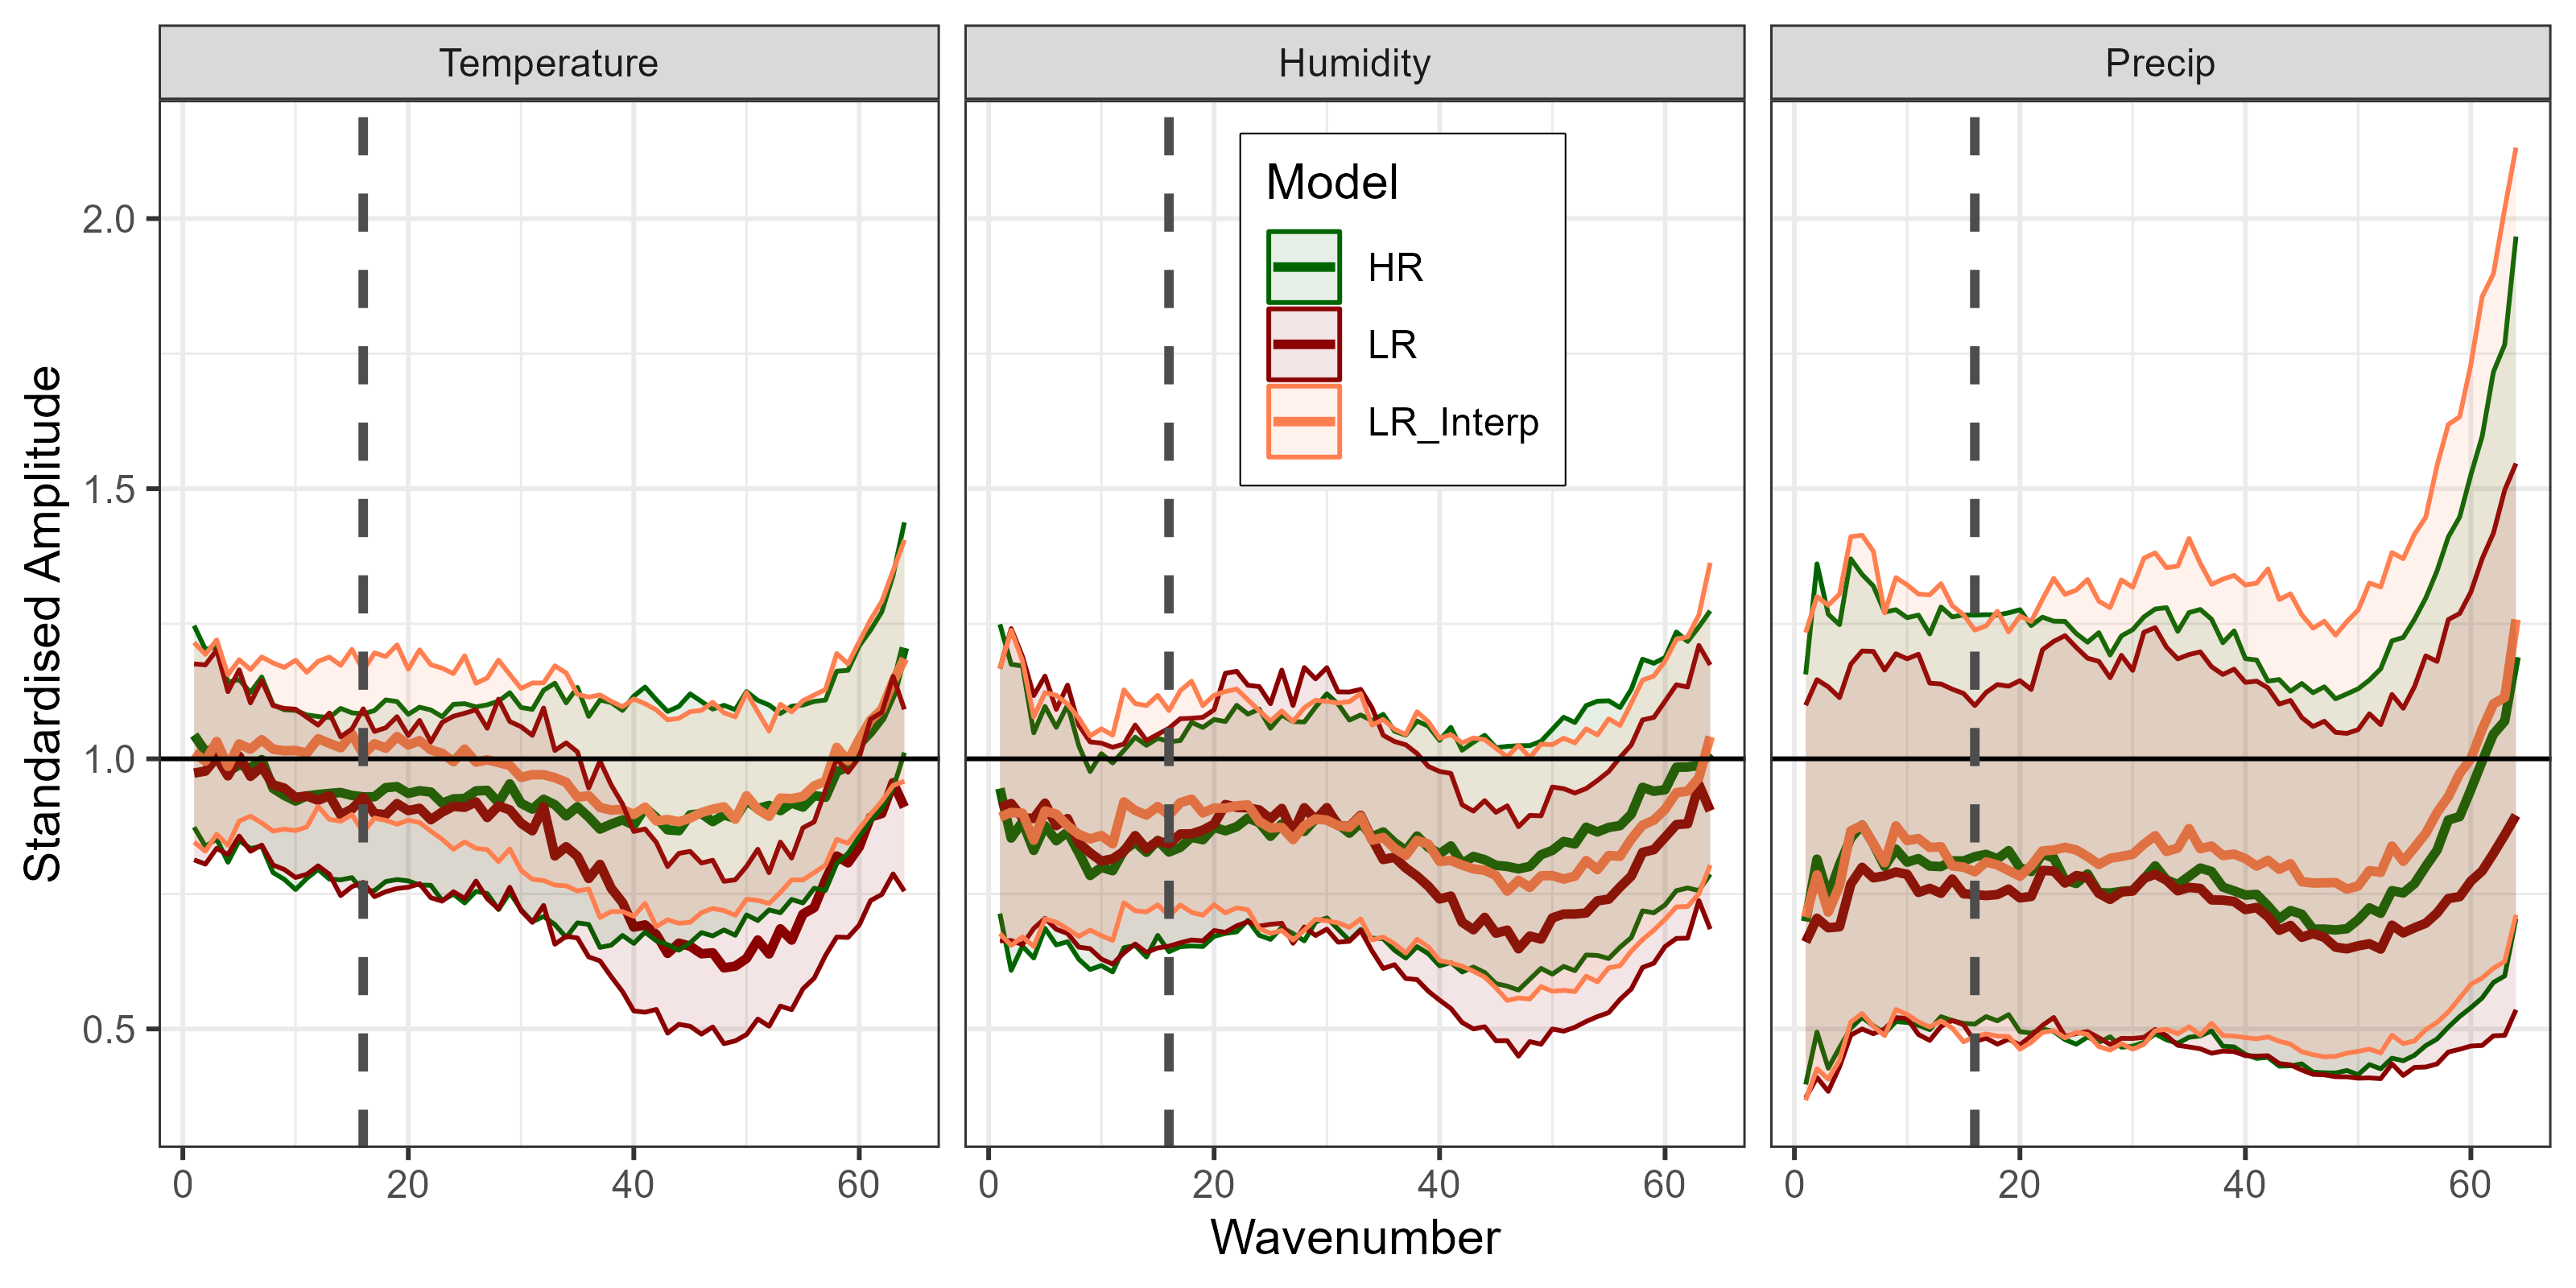
\includegraphics[width=\textwidth,angle=0]{final/RASP_TopoExp.png}\\
  \caption{Median and IQR RASP for temperature,  humidity, and precipitation using HR topography, interpolated LR topography, and LR topography. Spectral powers are standardised to ground truth fields, and metrics are calculated across 1200 randomly selected fields. Dashed line shows wavenumber corresponding to LR grid size.}\label{hr_topo}
\end{figure}

\subsection{Generalisation Across Space}
Downscaling in the Northeast region was successful for certain variables, but showed more challenges than in the Coastal region (figure \ref{location2}). Downscaling of wind components showed similar quality to the Coastal region, whereas generated temperature and humidity fields often showed substantial differences from WRF. This was especially apparent for humidity, where generated fields were overly smooth and lacked a lot of the fine-scale details of WRF. Precipitation showed the most challenges; generated fields often had entirely different structure than the WRF field. The fourth row in figure \ref{location2} shows a representative sample of precipitation, with the generated fields showing patchy, high intensity precipitation across the domain. 

Most variables showed a substantial difference in the large-scale structure of the ERA5 field compared to the WRF field. This was especially apparent for precipitation; for the sample in figure \ref{location2}, the WRF field shows low-intensity precipitation through much of the field, while the ERA5 field shows a concentrated area of precipitation near the centre. To determine if this mismatch between the LR and HR fields was responsible for the poor downscaling quality, we trained a model where the LR precipitation field was created by coarsening the WRF field, resulting in zero bias in the large scale structure. This model produced substantially more accurate downscaling, with generated precipitation patterns closely matching the WRF field (fifth row of figure \ref{location2}).

Covariate choice was especially important in this region; we found that CAPE was an important covariate for all variables in this region, whereas in the coastal region, CAPE had only improved results for precipitation. 

\begin{figure}[H]
  \noindent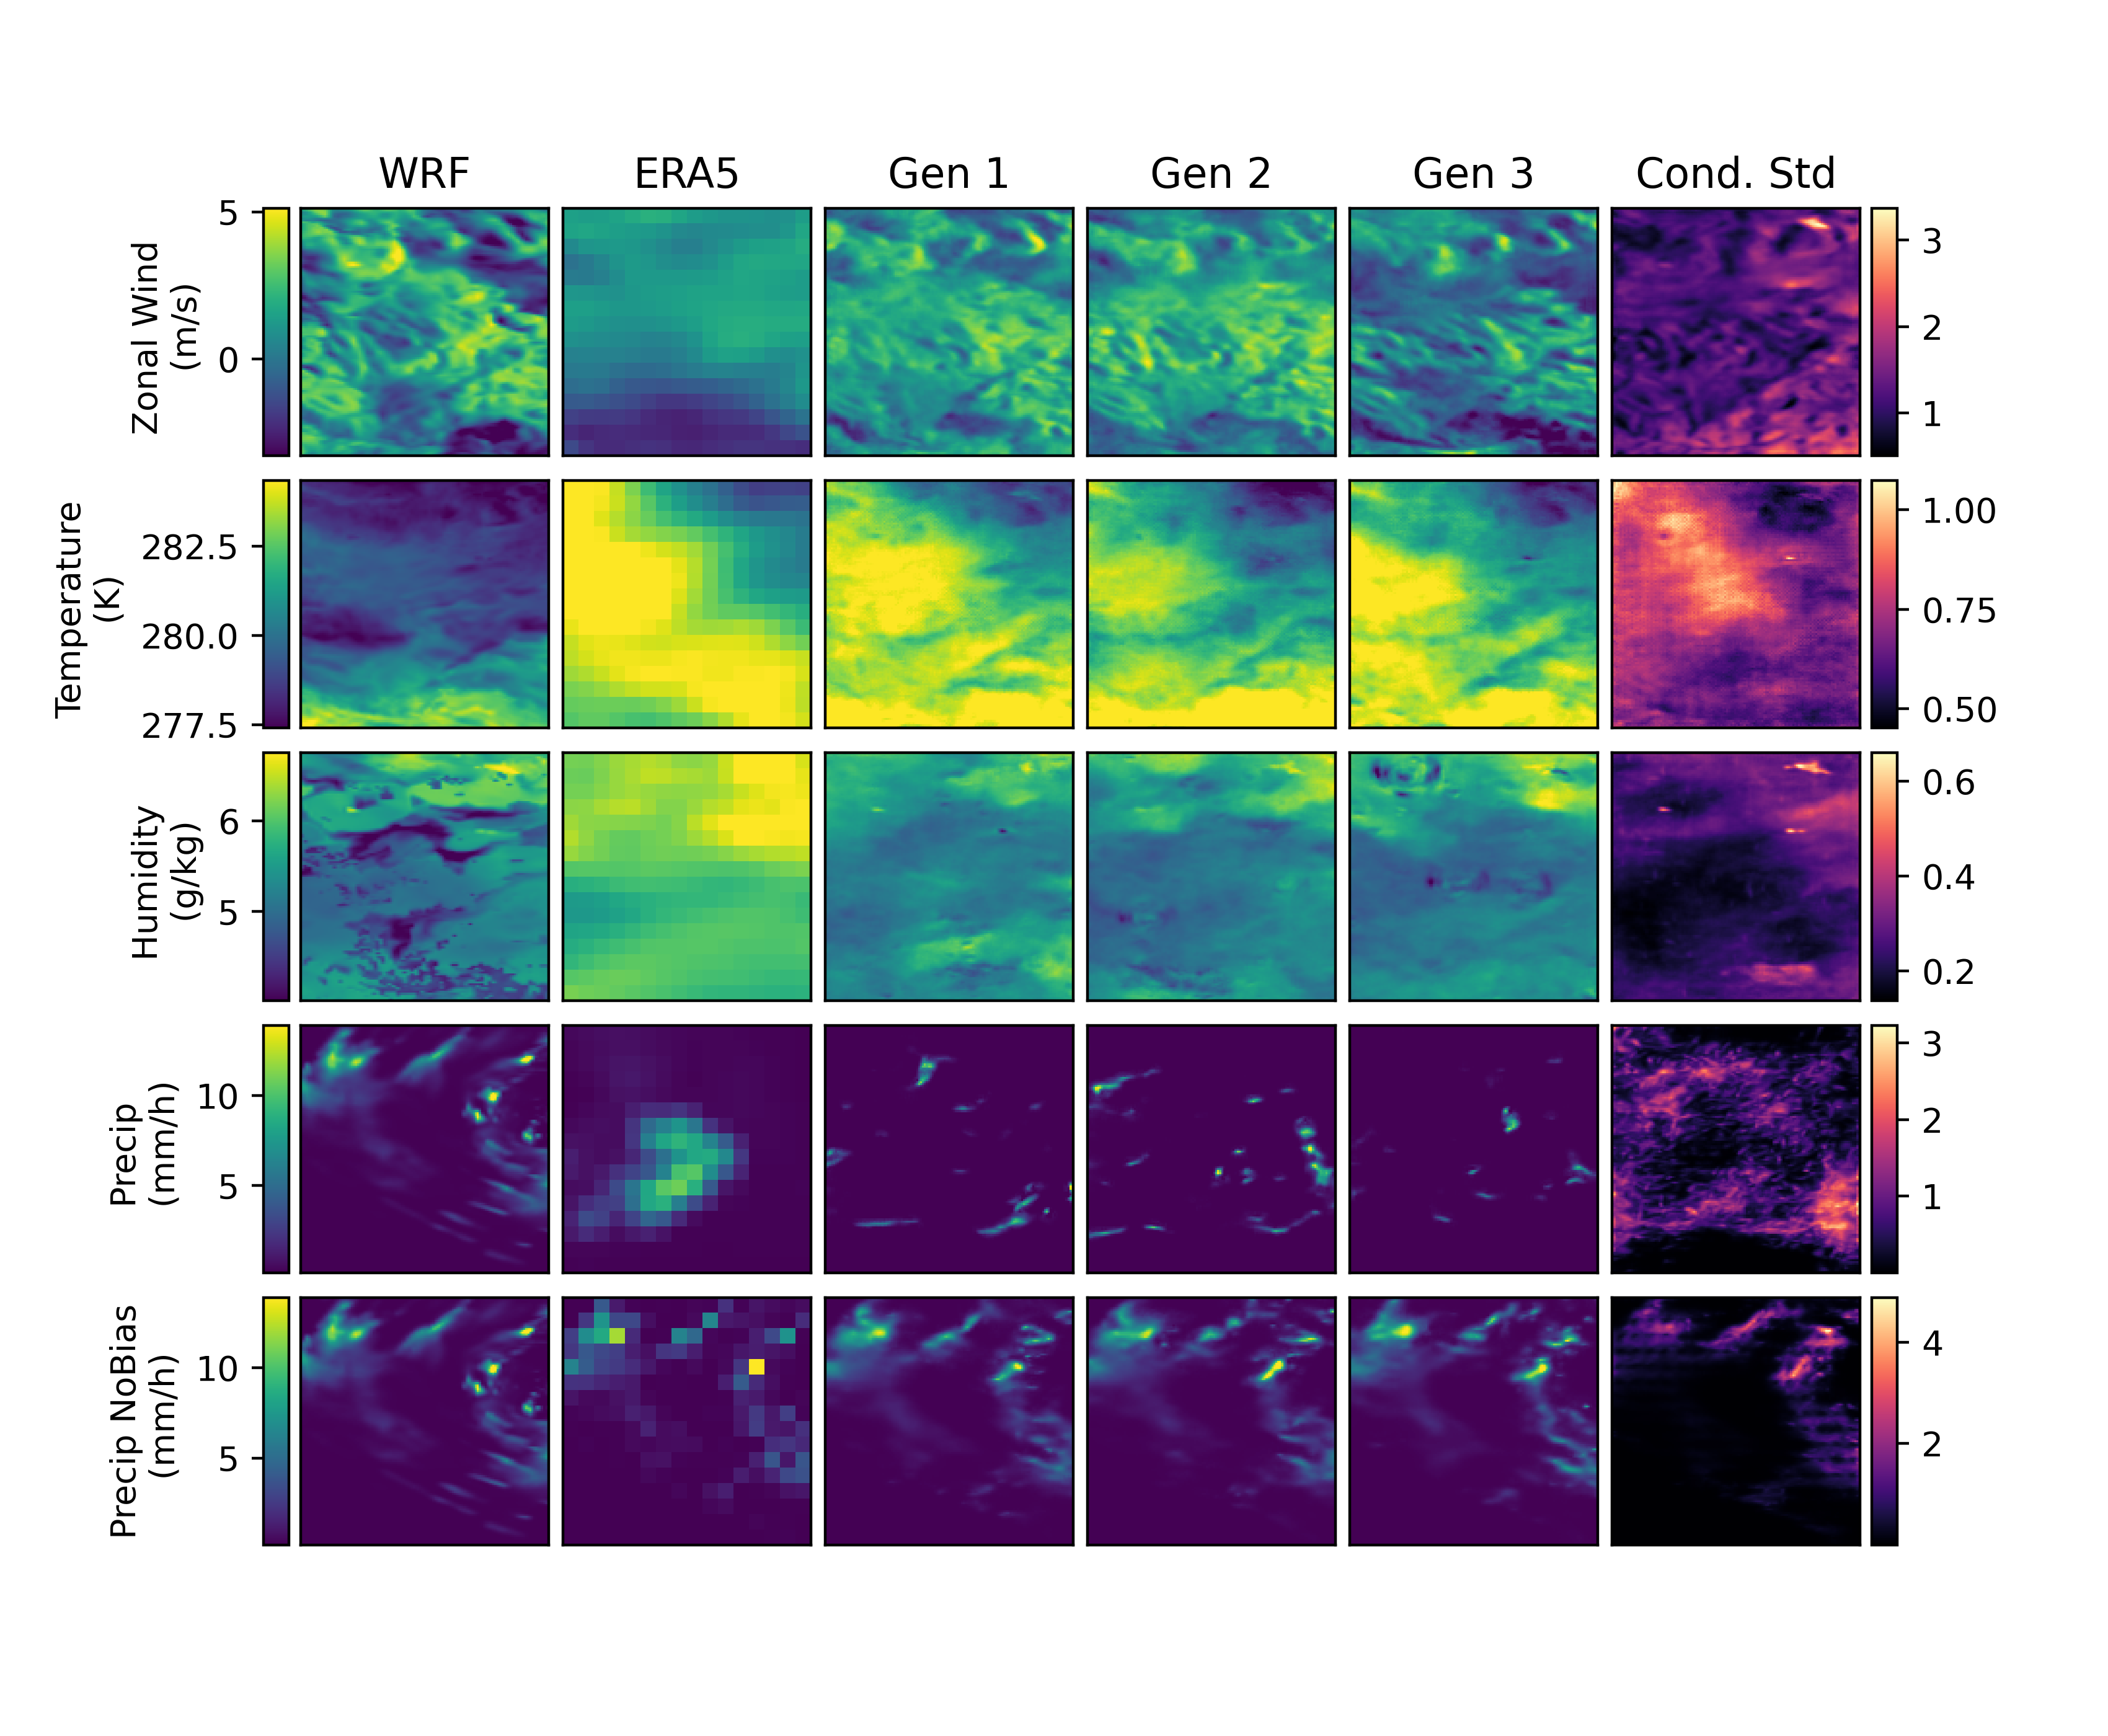
\includegraphics[width=\textwidth,angle=0]{final/Loc2_Allvars_2Precip.png}\\
  \caption{Example realisations for the Northeastern region. Rows correspond to variables, and the bottom row shows a second precipitation model with no bias between the LR and HR training data. Columns show, from left to right, WRF (i.e. ground truth), ERA5 (input conditioning field), three generated realisations, and the conditional standard deviations across 500 realisations }\label{location2}
\end{figure}

Stochastic calibration of conditional distributions was worse for temperature, humidity and standard precipitation in the Northeast region than in the Southwest region (figure \ref{loc2_rankhist}). Temperature and humidity both showed underdispersion, with many true samples falling outside the generated range, and precipitation showed underestimation, as many true samples fell above the generated range. The unbiased precipitation model had much better calibration than the standard precipitation model, and was one of the best calibrated models overall. Wind components showed similar calibration to the Coastal location. 
\begin{figure}[H]
  \noindent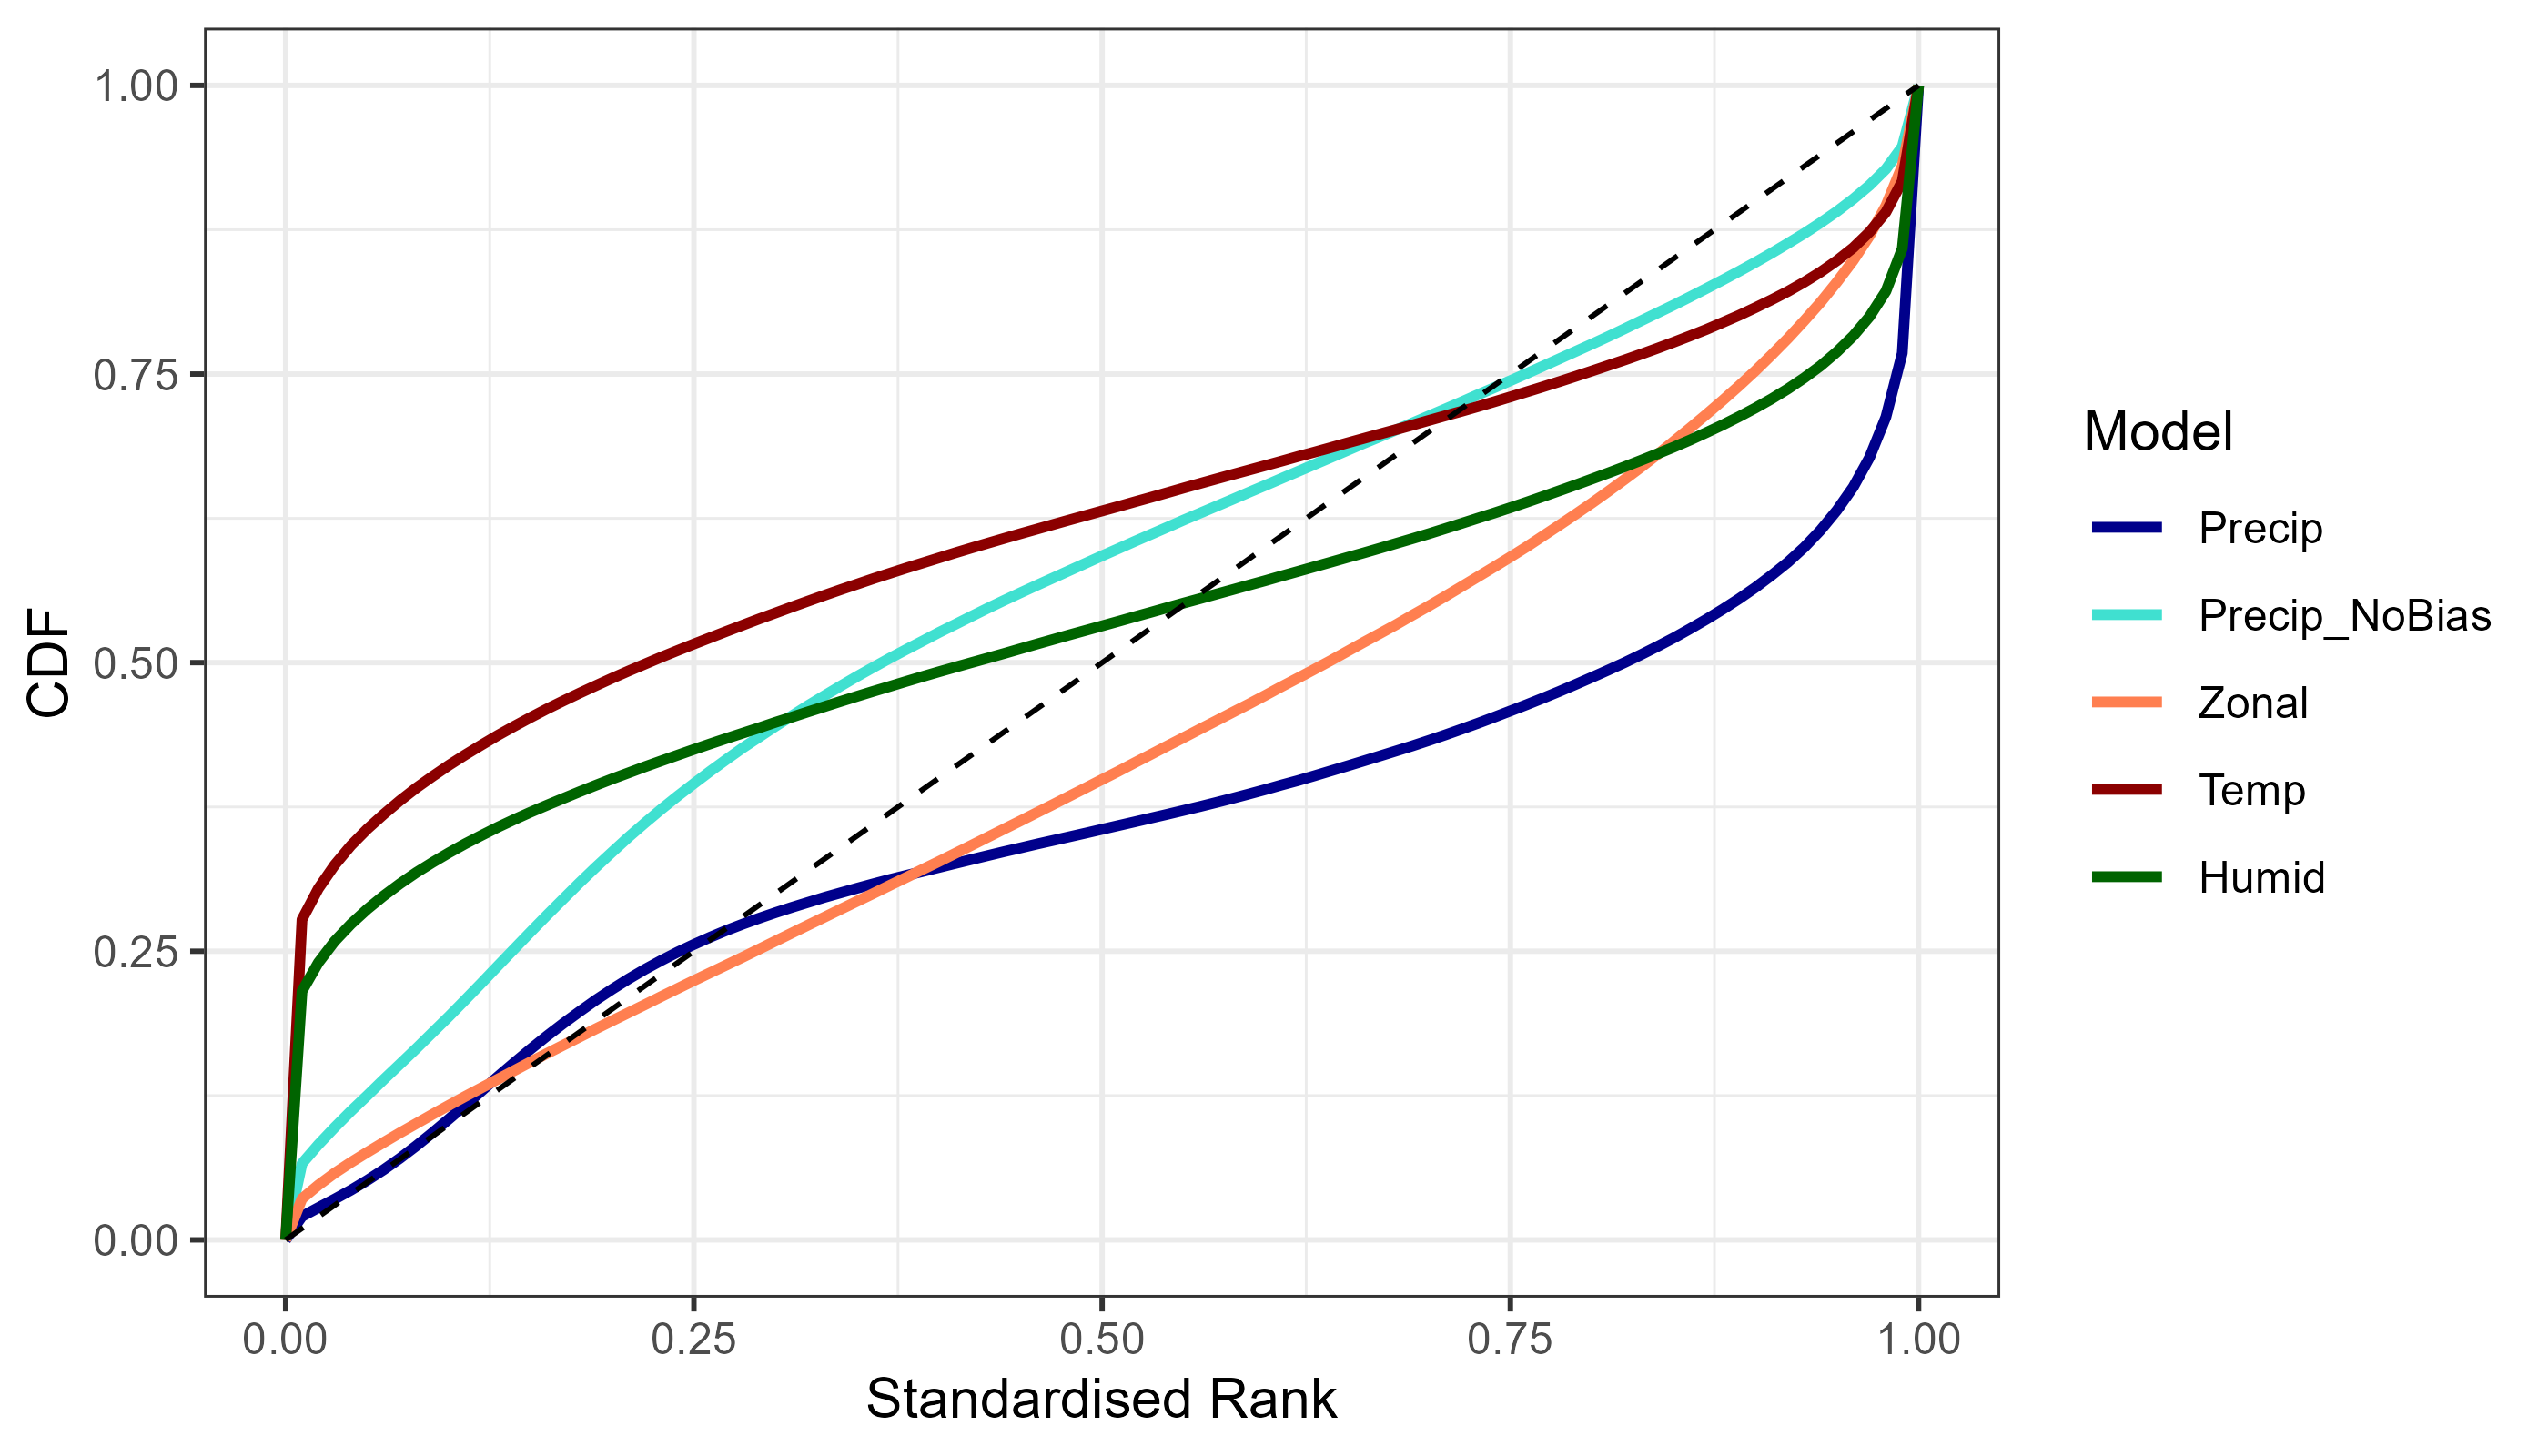
\includegraphics[width=0.5\textwidth,angle=0]{final/Location2_RankHist.png}\\
  \caption{CDFs of rank histograms showing stochastic calibration of models in the Northeastern region. Rank histograms were calculated across 100 randomly selected conditioning fields, with 96 HR realisations of each. Dashed line shows reference uniform CDF.}\label{loc2_rankhist}
\end{figure}
RASP metrics for variables in the Northeast region showed similar median values for humidity, temperature, and wind compared to the Coastal region, but had much larger inter-quantile ranges, representing more variability in texture bias between samples (figure \ref{loc2_rasp}). The standard precipitation model showed substantial low-power bias across scales, but especially at low wavenumbers where power was less than 50\% of corresponding WRF power. Conversely, the unbiased precipitation model showed good calibration over most of the range, and much smaller IQR. 
\begin{figure}[H]
  \noindent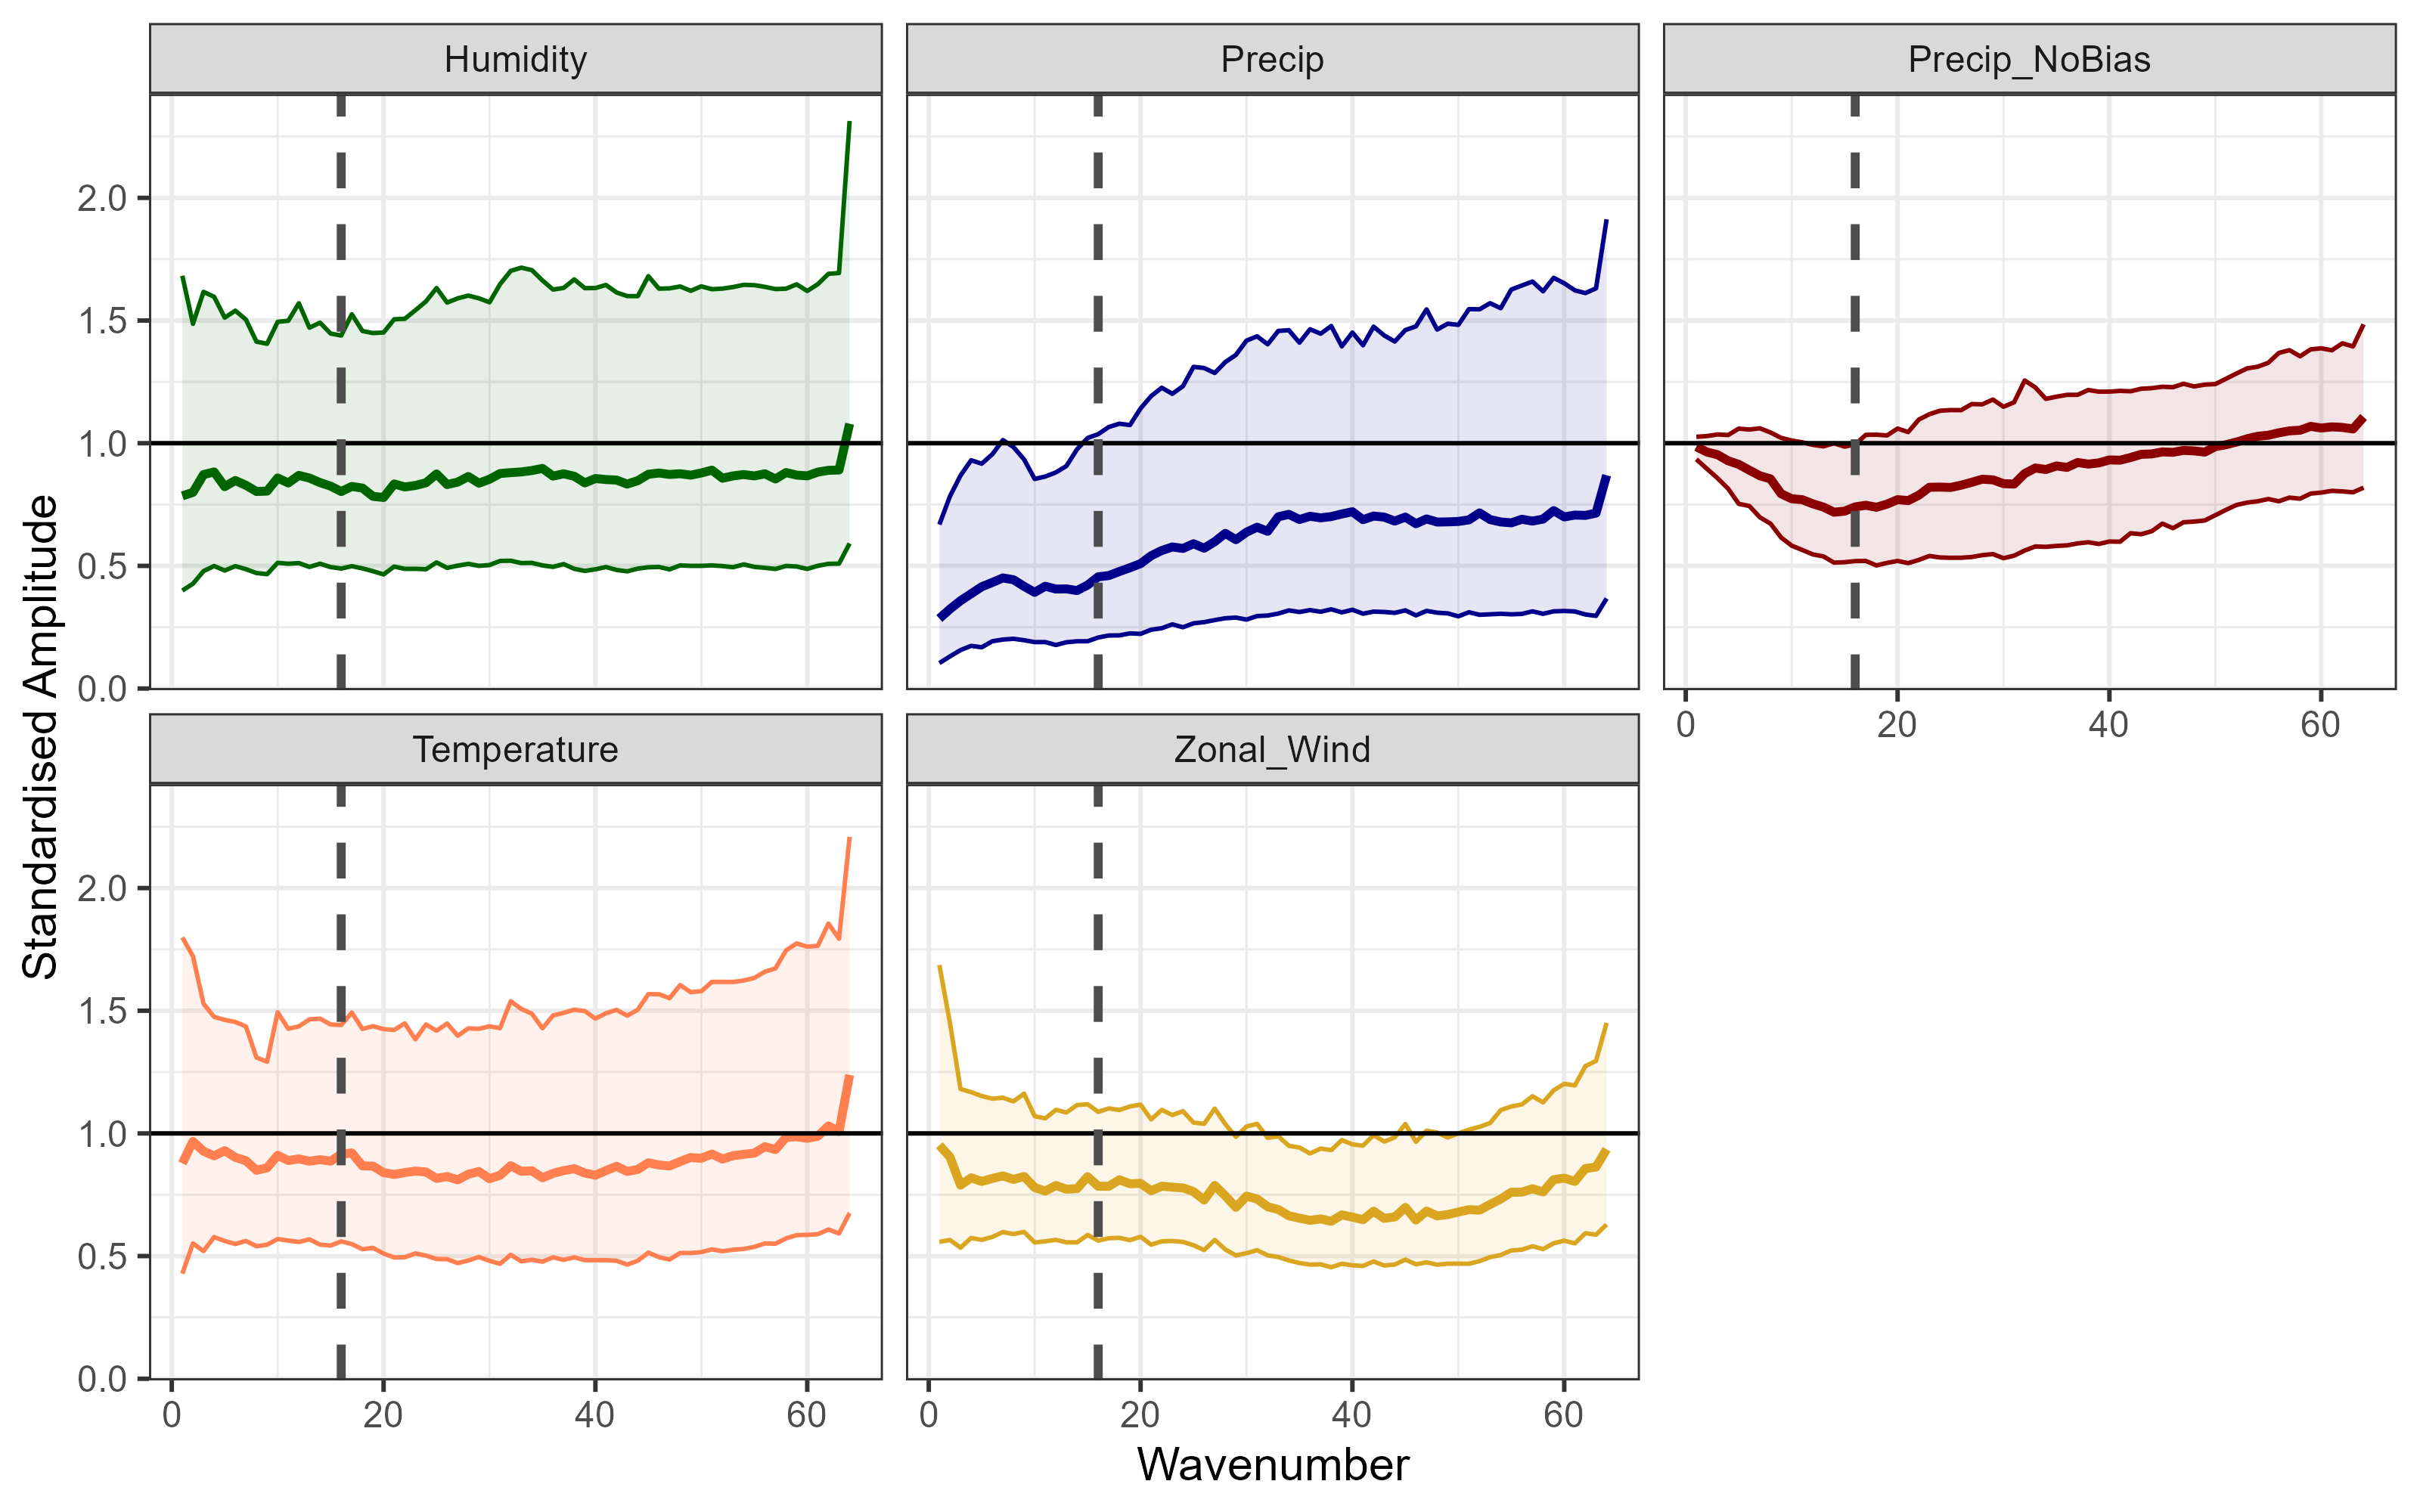
\includegraphics[width=\textwidth,angle=0]{final/Loc2_RASP_Precip_Coarsened.png}\\
  \caption{RASP humidity, precipitation, temperature, and zonal wind in the Northeast region, showing median and inter quartile ranges. Spectral powers are standardised to ground truth fields, and metrics are calculated across 1200 randomly selected fields.}\label{loc2_rasp}
\end{figure}

\section{Discussion}

This paper investigates practical considerations of applying the stochastic GAN framework from \citet{daust2024capturing} to realistic downscaling applications. Specifically, we focus on extension of GANs to multiple climate variables, including the applicability of multivariate prediction, and generalisability to different locations. We show that the stochastic GAN framework can successfully downscale a suite of variables. We then find that while multivariate downscaling improves the dependence structures of downscaled variables, it tends to decrease the quality of individual downscalings. Finally, we show mixed success in generalising to the Northeast region: models for temperature, humidity, and wind components produced reasonable downscalings, but were less accurate than in the Southwest region. Precipitation models struggled in this region, likely due to large-scale biases between the LR and HR training data.

\subsection{Extension to temperature, humidity, and precipitation}
Overall, we found that the stochastic GAN successfully downscaled temperature, specific humidity, and precipitation, although it was less accurate with humidity than the other variables. Challenges with downscaling humidity could be due to a variety of reasons. First, WRF humidity fields often showed very sharp gradients around valleys, which the GAN often did not capture fully. It may also be that we did not include all important covariates; for example, it would be interesting to add temporal pressure gradients as a LR covariate. 

Precipitation is an important variable, and is often more challenging to downscale due to its unusual distribution. We show that the stochastic GAN performs well at downscaling precipitation, and is much better at capturing extreme precipitation events than a deterministic GAN. Since extremely heavy precipitation is likely to cause flooding and damage, being able to capture it is important. This result supports the finding of \citet{daust2024capturing}, who show that by sampling from the full HR distribution, the stochastic GAN was better able to estimate wind component extremes. 

\subsection{Multivariate Prediction}
Multivariate predication lead to improved dependence structure between dependant variables, but decreased the quality of predictions of individual variables. It seems reasonable that for variables with strong dependence, multivariate prediction would lead to better consistency, as it allows fine-scale variability to be harmonised between variables. For temperature and humidity, multivariate models generated fields with mutual information scores closer to that of the WRF variables. However, variables generated from the full multivariate model were noticeably more blurry, failed to capture fine scale variability, and showed artifacts. Humidity seemed especially challenging; the univariate model was the only model able to recreate the fine-scale features around the Straight of Georgia, and the full multivariate model created predictions still showing artifacts of the convolutional filters. When we removed precipitation from the model and only predicted wind components, temperature, and humidity, results were improved, but still blurry. Precipitation has a very different distribution than the other variables; it seems that trying to predict variables with different distributions in challenging. Perhaps since the convolutional filters being learned for each field are so different, the final result is an overall poorer compromise. However, it is interesting that even with precipitation removed, generated fields were less accurate. Using multivariate prediction means that there are fewer tunable parameters that can be used specifically for a single variable. We hypothesise that this may lead to decreased flexibility for the model to adapt to a specific variable. An interesting avenue of future research would investigate whether adjusting the model architecture to improve flexibility could improve multivariate prediction. For example, it may be beneficial to separate the network in to separate branches near the end for each variable being prediction. In practice, it may still be advisable to use multivariate prediction for highly coupled variables (e.g., temperature and humidity, wind components), and univariate prediction for less dependant variables (e.g., precipitation). 

\subsection{HR Topography}
Including HR topography in the Generator improved spatial structures of wind components, temperature, and humidity, particularly at high wavenumbers. However, including LR interpolated topography produced downscaling of approximately similar quality, thus suggesting that network architecture may be more important than the topography resolution itself. Adding an HR input stream results in a substantially larger network, with more learnable weights at HR scales, especially since our architecture applies a RRDB to the HR input stream. Thus, even if the input has the same information, difference in architecture and the increased network size at the fine scales could allow the model to better capture fine scale details. It is interesting to note that the GANs with HR topography seemed to stabilise faster during training than the model with LR interpolated topography. This suggests that, given the correct architecture, the model can learn HR details over time, but is aided initially by having the HR information. For precipitation in the Northeast region, we also found that including a second HR covariate (land use index) improved predictions. However, since this addition slightly altered the network architecture, it is unclear whether the land use information itself was useful. Although adding a HR stream to the Generator increases network size, we believe that the substantial improvement in fine-scale structure makes this trade off worthwhile, and we suggest including HR covariates when possible.

\subsection{Generalisation in Space}
Applying the stochastic GAN framework to the Northeast location showed mixed success. Wind component downscalings generally showed similar high-accuracy as in the Southwest region. Temperature and humidity downscalings were reasonable but not as accurate, and precipitation models were initially poor, with generated fields showing very different spatial structure than the WRF fields. We hypothesise that some of the challenges in this region, especially with precipitation, were due to larger biases between WRF and ERA5 structures at large scales. It was visually apparent that in many samples, the LR conditioning fields did not match the structure of the corresponding WRF fields. Our unbiased precipitation model, where we created the LR conditioning fields by coarsening the WRF fields produced highly accurate downscaling, supporting our hypothesis that this mismatch is a source of the challenges. Unfortunately, in an operational setting, it is generally not possible to have unbiased LR and HR fields, as the HR fields do not exist. Some studies have already investigated the challenge of large-scale biases between datasets. \citet{price2022increasing} developed a GAN with two stages, the first to correct biases, and the second to downscale. However, this approach is only applicable if biases are consistent across samples. If biases change between samples, which we hypothesise is often true with precipitation, it becomes a much more challenging problem. Some of the challenges we found in this region may be improved by using a larger training region; biases between LR and HR data are likely more severe at smaller scales, and by using a larger area, there may be more consistency between datasets, resulting in increased stability during training. In regions with substantial bias, it may also be possible to train models using the unbiased coarsened data, and then predict using the bias LR dataset. While this technique would then not perform any bias correction, it could perform better at downscaling than an unstable model.

We noticed that covariate choice had a large effect on downscaling accuracy in the Northeast region compared to the Southwest region. Certain covariates, which had not been necessary in the Southwest region, were important for accurate downscaling in the Northeast. Convective Available Potential Energy was important for predicting precipitation, humidity, temperature, and wind components. While we included CAPE as a covariate in our final models for both regions, CAPE only improved precipitation downscaling on the Southwest region, whereas it improved all variables in the Northeast region. Since substantial fine-scale variability can result from convection, especially in regions of flatter topography, it makes sense that CAPE is an important variable in this region. In general, different suites of LR covariates will be needed depending on the downscaling region. Therefore, to obtain accurate downscalings over large areas, it will likely be necessary to include more covariates than required for a smaller region, as all subdomains will require the covariates important for their specific weather patterns.

\section{Conclusions}
It is becoming increasingly common for governments, industries, and other organisations to use downscaled climate data for modelling, planning, and adaptation purposes. Most of downscaled products easily available do a poor job at capturing climatic extremes, which are arguably the most important (ref xxx). Deep-learning downscaling is a promising method for improving this challenge, as it provides a computationally efficient way of downscaling LR model output to convection-permitting scales, thus better capturing extremes. While substantial research has occurred in this field recently, deep-learning downscaling has not be been used in a large operational setting. This paper addresses some of the challenges inherent in applying GAN based downscaling operationally. We show that the stochastic GAN framework can be extended to a suite of important variables, that including HR covariates increases accuracy, and that while the framework can be applied to a different region, there are some challenges related to large-scale bias between HR and LR fields. A final step required for operational GANs will involve overcoming the computational challenges linked to training on large spatial regions. Tiling methods, which have been applied in other deep-learning and computer vision settings, will be an important avenue of future research. Hopefully, GAN downscaling will soon be an important tool for climate adaptation.
%%%%%%%%%%%%%%%%%%%%%%%%%%%%%%%%%%%%%%%%%%%%%%%%%%%%%%%%%%%%%%%%%%%%%
% TABLES---INSERT NEAR IN-TEXT DISCUSSION
%%%%%%%%%%%%%%%%%%%%%%%%%%%%%%%%%%%%%%%%%%%%%%%%%%%%%%%%%%%%%%%%%%%%%
%%  Enter tables near where they are discussed within the document. 
%%  Please place tables before/after paragraphs, not within a paragraph.
%%
%
%\begin{table}[t]
%\caption{This is a sample table caption and table layout.  Enter as many tables as
%  necessary at the end of your manuscript. Table from Lorenz (1963).}\label{t1}
%\begin{center}
%\begin{tabular}{ccccrrcrc}
%\hline\hline
%$N$ & $X$ & $Y$ & $Z$\\
%\hline
% 0000 & 0000 & 0010 & 0000 \\
% 0005 & 0004 & 0012 & 0000 \\
% 0010 & 0009 & 0020 & 0000 \\
% 0015 & 0016 & 0036 & 0002 \\
% 0020 & 0030 & 0066 & 0007 \\
% 0025 & 0054 & 0115 & 0024 \\
%\hline
%\end{tabular}
%\end{center}
%\end{table}

%%%%%%%%%%%%%%%%%%%%%%%%%%%%%%%%%%%%%%%%%%%%%%%%%%%%%%%%%%%%%%%%%%%%%
% FIGURES---INSERT NEAR IN-TEXT DISCUSSION
%%%%%%%%%%%%%%%%%%%%%%%%%%%%%%%%%%%%%%%%%%%%%%%%%%%%%%%%%%%%%%%%%%%%%
%%  Enter figures near where they are discussed within the document.
%%  Please place figures before/after paragraphs, not within a paragraph.
% %
%
%\begin{figure}[t]
%  \noindent\includegraphics[width=19pc,angle=0]{figure01.pdf}\\
%  \caption{Enter the caption for your figure here.  Repeat as
%  necessary for each of your figures. Figure from \protect\cite{Knutti2008}.}\label{f1}
%\end{figure}

\clearpage
%%%%%%%%%%%%%%%%%%%%%%%%%%%%%%%%%%%%%%%%%%%%%%%%%%%%%%%%%%%%%%%%%%%%%
% ACKNOWLEDGMENTS
%%%%%%%%%%%%%%%%%%%%%%%%%%%%%%%%%%%%%%%%%%%%%%%%%%%%%%%%%%%%%%%%%%%%%
\acknowledgments
%  Keep acknowledgments (note correct spelling: no ``e'' between the ``g'' and
% ``m'') as brief as possible. In general, acknowledge only direct help in
%  writing or research. Financial support (e.g., grant numbers) for the work done, 
%  for an author, or for the laboratory where the work was performed must be 
%  acknowledged here rather than as footnotes to the title or to an author's name.
%  Contribution numbers (if the work has been published by the author's institution 
%  or organization) should be placed in the acknowledgments rather than as 
%  footnotes to the title or to an author's name.

%%%%%%%%%%%%%%%%%%%%%%%%%%%%%%%%%%%%%%%%%%%%%%%%%%%%%%%%%%%%%%%%%%%%%
% DATA AVAILABILITY STATEMENT
%%%%%%%%%%%%%%%%%%%%%%%%%%%%%%%%%%%%%%%%%%%%%%%%%%%%%%%%%%%%%%%%%%%%%
% 
%
\datastatement
%  The data availability statement is where authors should describe how the data underlying 
%  the findings within the article can be accessed and reused. Authors should attempt to 
%  provide unrestricted access to all data and materials underlying reported findings. 
%  If data access is restricted, authors must mention this in the statement. See
%  {http://www.ametsoc.org/PubsDataPolicy} for more info.

%%%%%%%%%%%%%%%%%%%%%%%%%%%%%%%%%%%%%%%%%%%%%%%%%%%%%%%%%%%%%%%%%%%%%
% APPENDIXES
%%%%%%%%%%%%%%%%%%%%%%%%%%%%%%%%%%%%%%%%%%%%%%%%%%%%%%%%%%%%%%%%%%%%%
%
%% If only one appendix, use

%\appendix

%% If more than one appendix, use \appendix[<letter>], e.g.,

%\appendix[A] 

%% Appendix title is necessary! For appendix title:

%\appendixtitle{Title of Appendix}

%%% Appendix section numbering (note, skip \section and begin with \subsection)
%
% \subsection{First primary heading}

% \subsubsection{First secondary heading}

% \paragraph{First tertiary heading}


%%%%%%%%%%%%%%%%%%%%%%%%%%%%%%%%%%%%%%%%%%%%%%%%%%%%%%%%%%%%%%%%%%%%%
% REFERENCES
%%%%%%%%%%%%%%%%%%%%%%%%%%%%%%%%%%%%%%%%%%%%%%%%%%%%%%%%%%%%%%%%%%%%%
% Make your BibTeX bibliography by using these commands:
\bibliographystyle{ametsocV6}
\bibliography{references}


\end{document}